\documentclass[12pt,oneside,a4paper,brazil,final]{abntex2}



% ----------------------------------------------------------

% PACOTES DE IDIOMA E FONTE

% ----------------------------------------------------------

\usepackage[brazil]{babel}



% Fonte Arial

% IMPORTANTE: no Overleaf, usar Menu -> Compiler -> XeLaTeX

\usepackage{fontspec}

\setmainfont{Arial}



\usepackage{microtype}

\usepackage{indentfirst}

\usepackage{setspace}

\usepackage{ragged2e}

\usepackage{url}

\usepackage{hyperref}



% ----------------------------------------------------------

% IMAGENS, TABELAS E CÓDIGOS

% ----------------------------------------------------------

\usepackage[final]{graphicx}

\usepackage{float}

\usepackage{array}

\usepackage{longtable}

\usepackage{booktabs}

\usepackage{caption}

\usepackage{listings}

\usepackage{xcolor}



% ----------------------------------------------------------

% MARGENS ABNT

% esquerda/superior 3 cm; direita/inferior 2 cm

% ----------------------------------------------------------

\usepackage[left=3cm,right=2cm,top=3cm,bottom=2cm]{geometry}



% ----------------------------------------------------------

% CENTRALIZAÇÃO VISUAL NA FOLHA

% Usado na capa e folha de rosto para centralizar CURITIBA/2026

% em relação à folha A4 inteira, e não apenas à área útil do texto.

% ----------------------------------------------------------

\newcommand{\centralizarfolha}[1]{%
\noindent\hspace*{-3cm}\makebox[\paperwidth][c]{#1}%
}





% ----------------------------------------------------------

% CONFIGURAÇÕES GERAIS DO TEXTO

% ----------------------------------------------------------

\setlength{\parindent}{1.5cm}

\setlength{\parskip}{0cm}

\OnehalfSpacing

\justifying

\sloppy

\emergencystretch=3em



% ----------------------------------------------------------

% REMOVE CABEÇALHO AUTOMÁTICO DO ABNTEX2

% Deixa somente o número da página no canto superior direito

% ----------------------------------------------------------

\makepagestyle{meuestilo}



% Cabeçalho sem texto, só número da página à direita

\makeevenhead{meuestilo}{}{}{\thepage}

\makeoddhead{meuestilo}{}{}{\thepage}



% Rodapé vazio

\makeevenfoot{meuestilo}{}{}{}

\makeoddfoot{meuestilo}{}{}{}



% Remove linha horizontal do cabeçalho

\makeheadrule{meuestilo}{\textwidth}{0pt}



% Aplica o estilo

\pagestyle{meuestilo}

\aliaspagestyle{chapter}{meuestilo}



% ----------------------------------------------------------

% NOMES DOS ELEMENTOS EM MAIÚSCULO

% ----------------------------------------------------------

\renewcommand{\contentsname}{SUMÁRIO}

\renewcommand{\listfigurename}{LISTA DE ILUSTRAÇÕES}

\renewcommand{\listtablename}{LISTA DE QUADROS}

\renewcommand{\figurename}{FIGURA}

\renewcommand{\tablename}{QUADRO}

\renewcommand{\bibname}{REFERÊNCIAS}

\renewcommand{\resumoname}{RESUMO}

\renewcommand{\lstlistingname}{CÓDIGO}

\renewcommand{\lstlistlistingname}{LISTA DE CÓDIGOS}



% Garante que o babel/abntex2 não volte os nomes para minúsculas

\addto\captionsbrazil{%
  \renewcommand{\contentsname}{SUMÁRIO}%
  \renewcommand{\listfigurename}{LISTA DE ILUSTRAÇÕES}%
  \renewcommand{\listtablename}{LISTA DE QUADROS}%
  \renewcommand{\figurename}{FIGURA}%
  \renewcommand{\tablename}{QUADRO}%
  \renewcommand{\bibname}{REFERÊNCIAS}%
  \renewcommand{\resumoname}{RESUMO}%
}



% ----------------------------------------------------------

% FORMATAÇÃO DOS TÍTULOS

% ----------------------------------------------------------

\renewcommand{\ABNTEXchapterfont}{\normalfont\bfseries}

\renewcommand{\ABNTEXchapterfontsize}{\normalsize}



\renewcommand{\ABNTEXsectionfont}{\normalfont}

\renewcommand{\ABNTEXsectionfontsize}{\normalsize}



\renewcommand{\ABNTEXsubsectionfont}{\normalfont}

\renewcommand{\ABNTEXsubsectionfontsize}{\normalsize}



\renewcommand{\ABNTEXsubsubsectionfont}{\normalfont}

\renewcommand{\ABNTEXsubsubsectionfontsize}{\normalsize}


% ----------------------------------------------------------
% FORMATAÇÃO DO SUMÁRIO
% Títulos primários em negrito; títulos secundários sem negrito
% ----------------------------------------------------------
\renewcommand{\cftchapterfont}{\normalfont\bfseries}
\renewcommand{\cftchapterpagefont}{\normalfont\bfseries}
\renewcommand{\cftsectionfont}{\normalfont}
\renewcommand{\cftsectionpagefont}{\normalfont}
\renewcommand{\cftsubsectionfont}{\normalfont}
\renewcommand{\cftsubsectionpagefont}{\normalfont}
\renewcommand{\cftsubsubsectionfont}{\normalfont}
\renewcommand{\cftsubsubsectionpagefont}{\normalfont}




% ----------------------------------------------------------

% CONFIGURAÇÃO DAS FIGURAS

% Título em cima e fonte embaixo

% ----------------------------------------------------------

\DeclareCaptionLabelFormat{figuraMaiuscula}{FIGURA #2}

\DeclareCaptionLabelFormat{tabelaMaiuscula}{QUADRO #2}



\captionsetup[figure]{font=normalsize,labelfont=normalfont,textfont=normalfont,justification=centering,singlelinecheck=false,position=above,labelformat=figuraMaiuscula}



\newcommand{\fontefigura}[1]{%
    \begin{center}
    {\fontsize{10}{12}\selectfont FONTE: #1}
    \end{center}
}





% Imagem opcional: se o arquivo ainda não foi enviado ao Overleaf,

% o documento compila com um quadro de aviso no lugar da figura.

\newcommand{\placeholderfigura}[2]{%
    \fbox{%
        \begin{minipage}[c][8cm][c]{0.45\textwidth}
        \centering
        \textbf{#2}\\[0.3cm]
        Inserir imagem: \texttt{#1}
        \end{minipage}%
    }%
}

\newcommand{\incluirprint}[2]{%
    \IfFileExists{#1}{%
        \includegraphics[width=0.43\textwidth,keepaspectratio]{#1}%
    }{%
        \placeholderfigura{#1}{#2}%
    }%
}

% ----------------------------------------------------------
% CONFIGURAÇÃO DAS TABELAS

% ----------------------------------------------------------

\captionsetup[table]{font=normalsize,labelfont=normalfont,textfont=normalfont,justification=centering,singlelinecheck=false,position=above,labelformat=tabelaMaiuscula}

\newcommand{\fontetabela}[1]{%
    \begin{center}
    {\fontsize{10}{12}\selectfont FONTE: #1}
    \end{center}
}

% ----------------------------------------------------------
% CONFIGURAÇÃO DO SQL

% ----------------------------------------------------------

\lstdefinelanguage{SQL}{keywords={CREATE,TABLE,PRIMARY,KEY,AUTOINCREMENT,NOT,NULL,UNIQUE,FOREIGN,REFERENCES,INTEGER,TEXT,REAL,DEFAULT},keywordstyle=\bfseries,sensitive=false,comment=[l]{--},morestring=[b]'}

\lstset{language=SQL,basicstyle=\ttfamily\fontsize{9}{11}\selectfont,columns=fullflexible,keepspaces=true,breaklines=true,breakatwhitespace=false,frame=single,numbers=left,numberstyle=\tiny\ttfamily,captionpos=t,tabsize=2,showstringspaces=false}

% ----------------------------------------------------------
% LINKS

% ----------------------------------------------------------

\hypersetup{colorlinks=true,linkcolor=black,citecolor=black,urlcolor=black}

% ----------------------------------------------------------
% DADOS DO TRABALHO

% ----------------------------------------------------------

\titulo{DESENVOLVIMENTO DE UM ASSISTENTE VIRTUAL POR COMANDO DE VOZ PARA APOIO À PRODUÇÃO MUSICAL INDEPENDENTE EM DISPOSITIVOS ANDROID}

\autor{CRISTIAN ALEX ANYAIPOMA LEON \\ FABIO ROGÉRIO MUNHOZ JUNIOR}

\local{CURITIBA}

\data{2026}

\instituicao{UNIVERSIDADE TUIUTI DO PARANÁ}

\tipotrabalho{Trabalho acadêmico}

\preambulo{Trabalho apresentado ao curso de Análise e Desenvolvimento de Sistemas da Universidade Tuiuti do Paraná como requisito avaliativo parcial da disciplina de Projeto Interdisciplinar.}



\begin{document}



\selectlanguage{brazil}

\frenchspacing



% ----------------------------------------------------------
% CAPA
% ----------------------------------------------------------
\begin{capa}
\thispagestyle{empty}

{\OnehalfSpacing
\fontsize{14}{16}\selectfont
\setlength{\parindent}{0cm}

\centralizarfolha{\bfseries UNIVERSIDADE TUIUTI DO PARANÁ}\par

\vspace{\baselineskip}

\centralizarfolha{\bfseries CRISTIAN ALEX ANYAIPOMA LEON}\par
\centralizarfolha{\bfseries FABIO ROGÉRIO MUNHOZ JUNIOR}\par

\vspace*{8.2cm}

\centralizarfolha{\bfseries TOUCHLESS: APLICATIVO DE APOIO À ORGANIZAÇÃO}\par
\centralizarfolha{\bfseries DE PROJETOS MUSICAIS POR COMANDO DE VOZ}\par

\vfill

\centralizarfolha{\bfseries CURITIBA}\par
\centralizarfolha{\bfseries 2026}\par

}

\end{capa}



% ----------------------------------------------------------
% FOLHA DE ROSTO
% ----------------------------------------------------------
\begin{folhaderosto}
\thispagestyle{empty}

{\OnehalfSpacing
\fontsize{14}{16}\selectfont
\setlength{\parindent}{0cm}

\centralizarfolha{\bfseries CRISTIAN ALEX ANYAIPOMA LEON}\par
\centralizarfolha{\bfseries FABIO ROGÉRIO MUNHOZ JUNIOR}\par

\vspace*{7.5cm}

\centralizarfolha{\bfseries TOUCHLESS: APLICATIVO DE APOIO À ORGANIZAÇÃO}\par
\centralizarfolha{\bfseries DE PROJETOS MUSICAIS POR COMANDO DE VOZ}\par

\vspace*{3cm}

\noindent\hspace*{8cm}%
\begin{minipage}{7.8cm}
\SingleSpacing
\justifying
\setlength{\parindent}{0cm}
\setlength{\parskip}{0cm}
\fontsize{10}{12}\selectfont

Trabalho apresentado ao curso de Análise e Desenvolvimento de Sistemas da Universidade Tuiuti do Paraná como requisito avaliativo parcial da disciplina de Projeto Interdisciplinar.

\vspace{0.4cm}

Orientadores: Profª. Patrícia Rucker de Bassi; Prof. Sérgio Luiz Marques Filho; Profª. Ângela Helena Zatti.

\end{minipage}

\vfill

\centralizarfolha{\bfseries CURITIBA}\par
\centralizarfolha{\bfseries 2026}\par

}

\end{folhaderosto}


% ----------------------------------------------------------

% RESUMO

% ----------------------------------------------------------

\begin{resumo}
\noindent
Este trabalho apresenta o desenvolvimento de um assistente virtual baseado em comandos de voz voltado ao apoio de músicos independentes durante o processo de produção musical em dispositivos Android. A solução reduziu interrupções no fluxo criativo por meio de funcionalidades como reconhecimento de comandos de voz, controle de gravações de áudio, organização de arquivos, reprodução de gravações, registro de histórico, apresentação de indicadores em dashboard e fornecimento de feedback ao usuário. O protótipo permite iniciar, pausar, retomar, encerrar, salvar, listar, reproduzir, organizar, nomear e excluir gravações, além de registrar as ações realizadas durante o uso da aplicação. A aplicação foi desenvolvida utilizando a linguagem Dart, o framework Flutter e banco de dados local SQLite, permitindo funcionamento parcialmente offline e armazenamento estruturado das informações. Também foi considerada uma arquitetura experimental voice-first, voltada à validação de recursos como gerenciamento centralizado da sessão de voz, captura de áudio em stream, processamento em tempo real e diagnóstico de eventos. A metodologia adotada foi baseada na Programação Orientada a Objetos, no desenvolvimento incremental e na modelagem UML, com a utilização de diagramas de caso de uso, classes, sequência, arquitetura e entidade-relacionamento. Como resultado, foi obtido um protótipo funcional, com interface simples, feedback visual e/ou auditivo, dashboard de indicadores e recursos voltados à melhoria da produtividade e organização de ideias musicais.

\vspace{\onelineskip}

\noindent
\textbf{Palavras-chave}: Assistente virtual; Comando de voz; Produção musical; Gravação de áudio; Android.
\end{resumo}



% ----------------------------------------------------------

% LISTA DE ILUSTRAÇÕES

% ----------------------------------------------------------

\cleardoublepage

\begin{center}

\textbf{LISTA DE ILUSTRAÇÕES}

\end{center}

\vspace{\onelineskip}



\makeatletter

\@starttoc{lof}

\makeatother



\cleardoublepage



\begin{center}

\textbf{LISTA DE QUADROS}

\end{center}

\vspace{\onelineskip}



\makeatletter

\@starttoc{lot}

\makeatother



\cleardoublepage



% ----------------------------------------------------------

% SUMÁRIO

% ----------------------------------------------------------

\begin{center}

\textbf{SUMÁRIO}

\end{center}

\vspace{\onelineskip}



\makeatletter

\@starttoc{toc}

\makeatother



\cleardoublepage



\textual

\OnehalfSpacing

% Força a remoção do cabeçalho automático depois do início da parte textual

\pagestyle{meuestilo}

\aliaspagestyle{chapter}{meuestilo}



% ----------------------------------------------------------

% 1 INTRODUÇÃO

% ----------------------------------------------------------

\chapter{INTRODUÇÃO}



O avanço das tecnologias digitais e a ampla disseminação de dispositivos móveis têm transformado significativamente a forma como atividades criativas são realizadas. No contexto da produção musical independente, smartphones e tablets passaram a desempenhar um papel importante, permitindo que músicos criem, gravem e organizem suas ideias de maneira prática e acessível.



Apesar desses avanços, ainda existem desafios relacionados ao fluxo de trabalho desses usuários. Durante o processo criativo, é comum que o músico precise interromper sua atividade principal para realizar tarefas operacionais, como iniciar uma gravação, salvar um arquivo, nomear um conteúdo ou localizar uma gravação anterior. Essas interrupções podem comprometer a continuidade do pensamento criativo, resultando na perda de ideias ou na redução da produtividade.



Além disso, as ferramentas atualmente disponíveis no mercado, como gravadores de áudio, aplicativos de anotações e assistentes virtuais genéricos, funcionam de forma isolada e nem sempre oferecem integração eficiente entre si. Em projetos de software, a compreensão adequada do problema e das necessidades do usuário é fundamental para orientar o desenvolvimento de soluções mais coerentes com o contexto de uso (Pressman; Maxim, 2016).


\textbf{A justificativa deste trabalho} está relacionada à necessidade de melhorar o processo de produção musical independente, especialmente no que diz respeito à fluidez criativa e à organização de ideias musicais. Atualmente, músicos enfrentam dificuldades relacionadas à constante interrupção de suas atividades para realizar tarefas operacionais, como iniciar gravações, localizar arquivos, renomear conteúdos ou organizar materiais gravados. Assim, o desenvolvimento de um assistente virtual específico para esse contexto, com recursos de gravação, organização, histórico, dashboard e feedback ao usuário, representa uma contribuição relevante tanto do ponto de vista tecnológico quanto do ponto de vista da experiência do usuário.


\textbf{O problema de pesquisa deste trabalho} pode ser definido pela seguinte questão: como desenvolver um assistente virtual baseado em comandos de voz que seja capaz de auxiliar músicos independentes de forma eficiente, reduzindo interrupções e melhorando a produtividade durante o processo de gravação e organização de ideias musicais?



Assistentes virtuais já existentes, como Google Assistant e Siri, embora possuam recursos de reconhecimento de voz, não são projetados especificamente para o contexto da produção musical independente, apresentando limitações no controle de gravações, na organização de conteúdos criativos e no acompanhamento do histórico de uso.



Diante desse cenário, torna-se evidente a necessidade de uma solução que integre funcionalidades de gravação, organização, controle por voz e visualização de informações em um único sistema. Nesse contexto, este trabalho propõe o desenvolvimento de um assistente virtual baseado em comandos de voz, voltado ao apoio de músicos independentes em dispositivos Android, com recursos para controle, organização e acompanhamento de gravações de áudio.



\textbf{O objetivo geral deste trabalho é} desenvolver um assistente virtual baseado em comandos de voz para dispositivos móveis Android, com o objetivo de auxiliar músicos independentes durante o processo de produção musical, proporcionando maior fluidez, praticidade e eficiência nas atividades de criação, gravação e organização de conteúdos sonoros.



\textbf{Os objetivos específicos deste trabalho são}: desenvolver um mecanismo de reconhecimento de comandos de voz; implementar funcionalidades para iniciar, pausar, retomar e encerrar gravações; permitir o salvamento automático dos arquivos de áudio; possibilitar a reprodução, listagem, renomeação, organização e exclusão das gravações; registrar o histórico de gravações, comandos e ações realizadas; implementar cadastro e autenticação de usuário; criar um dashboard com indicadores de uso, como quantidade de gravações realizadas, gravações reproduzidas, comandos executados e gravações excluídas; fornecer feedback visual e/ou auditivo ao usuário; e desenvolver uma interface simples e intuitiva para dispositivos Android.







\textbf{A delimitação do projeto} compreende o desenvolvimento de um sistema voltado para dispositivos móveis com sistema operacional Android. O sistema terá como foco o controle de gravações de áudio por comandos de voz, a organização dos arquivos, o registro de histórico, o fornecimento de feedback ao usuário e a apresentação de indicadores em dashboard. Não serão contempladas, nesta etapa, funcionalidades avançadas de edição musical profissional, mixagem multipista, aplicação de plugins externos, colaboração em tempo real entre usuários, armazenamento em nuvem ou recursos de edição detalhada de áudio.



Como produtos gerados, este trabalho apresenta a documentação de requisitos, modelagem UML, modelagem de dados, scripts de criação do banco de dados, telas do protótipo, fluxo de navegação de telas, relatório de testes e validações, demonstração de resultados a partir do programa implementado, protótipo funcional da aplicação Android, recursos de gravação e organização de áudio, e código-fonte versionado em repositório digital. O manual técnico de instalação, execução e uso do protótipo encontra-se em apêndice deste trabalho.




% ----------------------------------------------------------

% 2 FUNDAMENTAÇÃO TEÓRICA

% ----------------------------------------------------------

\chapter{FUNDAMENTAÇÃO TEÓRICA}



Este capítulo apresenta os principais conceitos teóricos relacionados ao desenvolvimento do sistema proposto. São abordados temas como assistentes virtuais, reconhecimento de voz, produção musical independente, desenvolvimento de aplicações móveis, banco de dados local e modelagem UML. Esses conceitos servem como base para compreender as decisões técnicas adotadas no projeto.



\section{ASSISTENTES VIRTUAIS}



Assistentes virtuais são sistemas computacionais desenvolvidos para auxiliar usuários na execução de tarefas por meio de interações simplificadas, que podem ocorrer por texto, voz ou outros meios de entrada. Esses sistemas buscam interpretar solicitações do usuário e executar ações de forma automatizada, reduzindo a necessidade de interação manual constante. No contexto da interação humano-computador, a redução de esforço durante o uso de um sistema contribui para melhorar a experiência do usuário e tornar a aplicação mais adequada às suas necessidades (Sommerville, 2019).



No contexto deste projeto, o assistente virtual tem como objetivo apoiar músicos independentes durante o processo de criação e gravação musical. Diferentemente de assistentes virtuais genéricos, a proposta do sistema está direcionada a um domínio específico: o controle de gravações de áudio, a organização de arquivos, o registro de histórico e a emissão de feedback ao usuário.



A utilização de um assistente virtual nesse contexto contribui para a redução de interrupções durante o fluxo criativo. Ao permitir que ações sejam executadas por comandos de voz, o usuário pode manter o foco em atividades como tocar instrumentos, cantar, compor ou testar ideias musicais, sem depender exclusivamente da manipulação manual da interface do aplicativo.



\section{RECONHECIMENTO DE VOZ}



O reconhecimento de voz é uma tecnologia que permite a captura e interpretação da fala humana por sistemas computacionais. Por meio dessa tecnologia, comandos emitidos oralmente podem ser convertidos em texto ou em instruções compreensíveis pelo sistema. Em aplicações móveis, esse tipo de recurso pode ser integrado para permitir formas alternativas de interação entre usuário e sistema, ampliando as possibilidades de uso da aplicação (Android Developers, 2026).



No sistema proposto, o reconhecimento de voz será utilizado para identificar comandos relacionados ao controle das gravações, como iniciar, pausar, retomar, encerrar, reproduzir, listar, excluir e nomear gravações. Dessa forma, a voz funciona como uma forma alternativa de entrada de dados e controle da aplicação.



Um dos desafios associados ao reconhecimento de voz é o tratamento de comandos não compreendidos ou interpretados de forma incorreta. Por esse motivo, o sistema deve prever fluxos de erro e mecanismos de feedback ao usuário, informando quando um comando não foi reconhecido e solicitando sua repetição. Esse tratamento é importante para tornar a aplicação mais confiável, clara e adequada ao uso em situações reais.



\section{PRODUÇÃO MUSICAL INDEPENDENTE}



A produção musical independente refere-se ao processo de criação, gravação, organização e publicação de músicas sem a dependência direta de grandes gravadoras ou estruturas profissionais tradicionais. Com o avanço das tecnologias digitais, músicos independentes passaram a utilizar computadores, dispositivos móveis, interfaces de áudio, aplicativos e plataformas digitais para desenvolver seus projetos musicais.



Nesse cenário, a organização das ideias musicais é um fator importante. Durante uma sessão criativa, o músico pode gerar melodias, letras, arranjos, linhas vocais, ideias de bateria, riffs ou trechos experimentais que precisam ser registrados rapidamente. Quando esse registro exige muitas etapas manuais, existe o risco de perda de concentração ou até mesmo de esquecimento da ideia original.



Assim, uma ferramenta voltada ao apoio da produção musical independente deve priorizar praticidade, rapidez e simplicidade. O sistema proposto busca atender essa necessidade ao permitir que o usuário controle gravações e organize arquivos por meio de comandos de voz, contribuindo para a continuidade do processo criativo.



\section{DESENVOLVIMENTO MOBILE COM FLUTTER}



O desenvolvimento de aplicações móveis exige a escolha de tecnologias adequadas ao público-alvo, ao sistema operacional utilizado e às funcionalidades necessárias. Neste projeto, a aplicação será desenvolvida para dispositivos Android, utilizando a linguagem Dart e o framework Flutter. A linguagem Dart é utilizada em conjunto com o Flutter para a construção da lógica da aplicação e da interface do sistema (Dart, 2026).



O Flutter é um framework voltado ao desenvolvimento de interfaces e aplicações multiplataforma. Sua utilização permite criar telas, componentes visuais, navegação entre páginas e integração com bibliotecas externas, sendo adequado para o desenvolvimento de protótipos funcionais e aplicações móveis. De acordo com a documentação oficial do Flutter, o framework possibilita o desenvolvimento de aplicações compiladas nativamente a partir de uma única base de código, utilizando a linguagem Dart (Flutter, 2026).



A escolha do Flutter se justifica pela possibilidade de desenvolver uma interface simples, responsiva e organizada, além de permitir integração com recursos importantes para o sistema, como reconhecimento de voz, gravação de áudio e armazenamento local. Dessa forma, a tecnologia atende às necessidades do projeto, especialmente no que se refere à criação de uma aplicação Android voltada à interação por voz.



\section{BANCO DE DADOS LOCAL}



O armazenamento de dados é uma parte essencial do sistema, pois permite registrar informações de usuários, gravações, arquivos de áudio, comandos de voz, histórico de ações, feedbacks e indicadores utilizados no dashboard. Para esse objetivo, o projeto utilizará um banco de dados local.



O SQLite é uma solução de banco de dados leve e adequada para aplicações móveis, pois permite armazenar dados diretamente no dispositivo do usuário. Essa característica contribui para o funcionamento parcialmente offline do sistema, evitando a dependência constante de conexão com a internet para acessar informações básicas da aplicação. Conforme a documentação oficial do SQLite, trata-se de uma biblioteca que implementa um mecanismo de banco de dados SQL incorporado, sem necessidade de um servidor separado (SQLite, 2026).



No contexto deste projeto, o banco de dados local será utilizado para armazenar os dados estruturados do sistema. As gravações terão seus dados registrados no banco, incluindo nome, data, duração, status e caminho do arquivo. Já os arquivos de áudio serão armazenados no dispositivo, com seus respectivos caminhos registrados para posterior consulta e reprodução. O banco também será responsável por registrar informações relacionadas aos comandos de voz, feedbacks, histórico de ações e indicadores utilizados no dashboard.



\section{MODELAGEM UML}



A UML, ou Linguagem de Modelagem Unificada, é utilizada para representar visualmente a estrutura e o comportamento de sistemas orientados a objetos. Segundo Booch, Rumbaugh e Jacobson (2006), a UML permite documentar, visualizar e especificar elementos de um sistema de software, auxiliando na comunicação entre os envolvidos no projeto.



Neste trabalho, a UML é utilizada para representar os principais aspectos do sistema proposto. O diagrama de caso de uso apresenta as funcionalidades disponíveis ao usuário. O diagrama de classes descreve a estrutura estática do sistema, indicando classes, atributos, métodos e relacionamentos. O diagrama de sequência representa a interação entre usuário, interface, assistente, reconhecimento de voz, controle de gravação, banco de dados, dashboard e feedback ao longo da execução das funcionalidades.



A utilização da modelagem UML contribui para organizar o desenvolvimento, reduzir ambiguidades e facilitar a compreensão do funcionamento do sistema antes da implementação. Além disso, os diagramas servem como documentação técnica do projeto, apoiando a validação dos requisitos e a comunicação entre os integrantes da equipe.



\section{ARQUITETURA VOICE-FIRST E PROCESSAMENTO EM TEMPO REAL}



A arquitetura voice-first corresponde a uma abordagem na qual a interação por voz passa a ocupar papel central no funcionamento do sistema. Nesse tipo de solução, o usuário pode executar comandos, controlar funcionalidades e receber feedback com menor dependência de interações manuais, favorecendo maior fluidez durante o uso da aplicação.



No contexto deste projeto, a arquitetura voice-first é aplicada ao controle de gravações e à organização de ações executadas pelo usuário. Além do reconhecimento de comandos de voz, o sistema passa a considerar aspectos como gerenciamento da sessão de voz, controle do uso do microfone, detecção de silêncio, tratamento de falhas e registro de eventos de diagnóstico.



Para reduzir riscos durante o desenvolvimento, a evolução voice-first será realizada de forma incremental. O fluxo principal de gravação e reconhecimento de voz permanece preservado, enquanto recursos experimentais, como captura de áudio em stream, processamento em tempo real, detecção adaptativa de silêncio e roteamento de eventos, são avaliados separadamente por meio de configurações específicas. Essa abordagem permite validar novas funcionalidades sem comprometer o funcionamento estável da aplicação.



% ----------------------------------------------------------

% 3 ANÁLISE DO SISTEMA ATUAL

% ----------------------------------------------------------

\chapter{ANÁLISE DO SISTEMA ATUAL}



No cenário atual, músicos independentes utilizam diversas ferramentas para apoiar o processo de criação musical, incluindo aplicativos de gravação de áudio, editores de texto, plataformas de organização de arquivos e assistentes virtuais genéricos. Embora essas ferramentas sejam úteis individualmente, elas não oferecem uma solução integrada, obrigando o usuário a alternar constantemente entre diferentes aplicações.



Essa fragmentação do processo impacta negativamente a experiência do usuário, especialmente em momentos de criação, nos quais a agilidade e a continuidade são essenciais. A necessidade de interromper uma atividade criativa para executar ações simples, como iniciar uma gravação, localizar um arquivo, renomear um áudio ou organizar uma ideia registrada, pode resultar na perda de ideias importantes.



Além disso, a interação com esses sistemas é predominantemente manual, o que exige atenção constante do usuário à interface do dispositivo. Isso representa uma limitação significativa, principalmente em situações em que o usuário está envolvido em atividades práticas, como tocar instrumentos musicais, cantar, compor ou testar arranjos.



Assistentes virtuais disponíveis no mercado apresentam recursos avançados de reconhecimento de voz, porém não são especializados no domínio da produção musical. Dessa forma, não oferecem suporte adequado para ações específicas, como controle detalhado de gravações, organização de sessões criativas, renomeação de arquivos de áudio e acompanhamento do histórico de uso.



Diante dessas limitações, observa-se a necessidade de uma solução capaz de integrar funcionalidades de gravação, organização, histórico, dashboard, feedback e interação por comandos de voz, permitindo maior eficiência, acessibilidade e melhor experiência ao usuário.



% ----------------------------------------------------------

% 4 LEVANTAMENTO DE REQUISITOS

% ----------------------------------------------------------

\chapter{LEVANTAMENTO DE REQUISITOS}



O levantamento de requisitos tem como objetivo identificar e definir as funcionalidades e restrições do sistema proposto. Esses requisitos são fundamentais para garantir que o sistema atenda às necessidades dos usuários e funcione de forma adequada.



Os requisitos foram divididos em requisitos funcionais, que descrevem as funcionalidades oferecidas pelo sistema, e requisitos não funcionais, que representam características de qualidade, desempenho, segurança e usabilidade.



\section{REQUISITOS FUNCIONAIS}



Os requisitos funcionais descrevem as ações que o sistema deve permitir ao usuário. Considerando a proposta do assistente virtual, os requisitos contemplam cadastro, autenticação, reconhecimento de comandos de voz, controle de gravações, organização de arquivos, feedback, histórico e dashboard, listados no Quadro~\ref{tab:requisitos-funcionais}.



\begin{longtable}{|p{2.3cm}|p{12cm}|}

\caption{REQUISITOS FUNCIONAIS DO SISTEMA}

\label{tab:requisitos-funcionais}\\

\hline

\textbf{Código} & \textbf{Descrição} \\

\hline

\endfirsthead



\hline

\textbf{Código} & \textbf{Descrição} \\

\hline

\endhead



RF01 & O sistema deve permitir o cadastro de usuários. \\

\hline

RF02 & O sistema deve permitir a autenticação de usuários por e-mail e senha. \\

\hline

RF03 & O sistema deve reconhecer comandos de voz do usuário. \\

\hline

RF04 & O sistema deve iniciar gravações de áudio por comando de voz. \\

\hline

RF05 & O sistema deve pausar gravações em andamento. \\

\hline

RF06 & O sistema deve retomar gravações pausadas. \\

\hline

RF07 & O sistema deve encerrar gravações quando solicitado. \\

\hline

RF08 & O sistema deve salvar automaticamente os arquivos de áudio. \\

\hline

RF09 & O sistema deve permitir a reprodução de gravações. \\

\hline

RF10 & O sistema deve fornecer feedback visual e/ou auditivo ao usuário. \\

\hline

RF11 & O sistema deve organizar os arquivos por data ou nome. \\

\hline

RF12 & O sistema deve permitir a exclusão de gravações. \\

\hline

RF13 & O sistema deve permitir a listagem das gravações existentes. \\

\hline

RF14 & O sistema deve permitir nomear gravações por comando de voz. \\

\hline

RF15 & O sistema deve registrar o histórico de gravações, comandos e ações realizadas. \\

\hline

RF16 & O sistema deve gerar um dashboard com indicadores de uso, como número de gravações realizadas, número de gravações reproduzidas, comandos executados e gravações excluídas. \\

\hline

\end{longtable}

\fontetabela{Autoria própria.}



\section{REQUISITOS NÃO FUNCIONAIS}



Os requisitos não funcionais descrevem as características de qualidade do sistema, considerando desempenho, compatibilidade, segurança, usabilidade, manutenção e funcionamento adequado dos recursos de gravação e organização de áudio.



\begin{longtable}{|p{2.3cm}|p{12cm}|}

\caption{REQUISITOS NÃO FUNCIONAIS DO SISTEMA}

\label{tab:requisitos-nao-funcionais}\\

\hline

\textbf{Código} & \textbf{Descrição} \\

\hline

\endfirsthead



\hline

\textbf{Código} & \textbf{Descrição} \\

\hline

\endhead



RNF01 & O sistema deve apresentar tempo de resposta inferior a 2 segundos para comandos simples. \\

\hline

RNF02 & O sistema deve possuir interface simples, intuitiva e acessível. \\

\hline

RNF03 & O sistema deve ser compatível com dispositivos Android versão 8 ou superior. \\

\hline

RNF04 & O sistema deve garantir estabilidade durante o uso. \\

\hline

RNF05 & O sistema deve consumir poucos recursos do dispositivo. \\

\hline

RNF06 & O sistema deve funcionar parcialmente offline. \\

\hline

RNF07 & O sistema deve garantir a integridade dos dados armazenados. \\

\hline

RNF08 & O sistema deve ser de fácil manutenção e atualização. \\

\hline

RNF09 & O sistema deve possuir boa usabilidade. \\

\hline

RNF10 & O sistema deve garantir segurança no armazenamento dos dados do usuário. \\

\hline

\end{longtable}

\fontetabela{Autoria própria.}



% ----------------------------------------------------------

% 5 METODOLOGIA

% ----------------------------------------------------------

\chapter{METODOLOGIA}

A metodologia adotada para o desenvolvimento deste projeto foi baseada na Programação Orientada a Objetos (POO), uma abordagem amplamente utilizada no desenvolvimento de sistemas devido à sua capacidade de promover organização, reutilização de código e facilidade de manutenção. A orientação a objetos favorece a organização do software em classes, objetos, atributos e métodos, facilitando a manutenção e a evolução do sistema (Booch; Rumbaugh; Jacobson, 2006). A escolha dessa metodologia se justificou pela necessidade de modelar entidades do sistema de forma estruturada, como usuário, gravação, arquivo de áudio, comando de voz, histórico, feedback e dashboard.

O processo de desenvolvimento seguiu um modelo incremental, no qual o sistema foi construído em etapas progressivas. Segundo Sommerville (2019), o desenvolvimento incremental permite que o sistema seja produzido em partes, possibilitando validações e ajustes ao longo do processo de construção. Cada etapa incluiu a implementação, teste e validação de funcionalidades específicas, permitindo ajustes contínuos e melhoria da qualidade do sistema. Inicialmente foram desenvolvidas as funcionalidades de cadastro e autenticação de usuário, seguidas pelo reconhecimento de voz, controle de gravações, armazenamento local, listagem de arquivos, histórico, feedback e dashboard.

O sistema foi desenvolvido utilizando a linguagem Dart e o framework Flutter. A escolha dessas tecnologias esteve relacionada à possibilidade de criação de aplicações móveis com interface responsiva, organização em componentes e uso de uma única base de código para diferentes plataformas, conforme descrito na documentação oficial do Flutter (Flutter, 2026). A escolha do Flutter se justificou por permitir o desenvolvimento de aplicações móveis para Android com boa organização de código, interface responsiva e facilidade de manutenção. Além disso, o framework oferece recursos adequados para criação de telas, navegação, integração com bibliotecas externas e desenvolvimento de protótipos funcionais. Essa característica foi importante para o projeto, pois permitiu integrar recursos relacionados ao reconhecimento de voz, gravação, reprodução e armazenamento local.

Para o armazenamento local dos dados, foi utilizado o banco de dados SQLite, por ser uma solução leve, integrada ao dispositivo móvel e adequada para aplicações Android que necessitam armazenar informações de forma offline. O SQLite é adequado para esse contexto por funcionar de forma incorporada à aplicação, sem exigir a instalação de um servidor de banco de dados separado (SQLite, 2026). O banco foi utilizado para registrar dados de usuários, gravações, arquivos de áudio, comandos reconhecidos, histórico de ações, feedbacks e informações utilizadas no dashboard.

\section{FERRAMENTAS UTILIZADAS}

Para o desenvolvimento do projeto, foram selecionadas ferramentas compatíveis com a proposta de criação de uma aplicação móvel Android com reconhecimento de voz, gravação de áudio, armazenamento local, interface simples e evolução gradual para uma arquitetura voice-first.

O Visual Studio Code foi utilizado como ambiente de desenvolvimento por permitir a edição do código-fonte, a organização dos arquivos do projeto e a integração com extensões voltadas ao desenvolvimento em Flutter e Dart. Essa ferramenta contribuiu para a produtividade da equipe e para a organização da implementação do protótipo.

A linguagem Dart foi utilizada por ser a linguagem principal do framework Flutter, possibilitando a construção da lógica da aplicação, dos componentes de interface e da navegação entre telas (Dart, 2026). O Flutter foi utilizado por permitir o desenvolvimento de aplicações móveis com interface responsiva, componentes reutilizáveis, integração com bibliotecas externas e geração de aplicativos para Android a partir de uma única base de código, sendo adequado à proposta do sistema (Flutter, 2026).

O Android SDK foi utilizado para compilar, executar e testar a aplicação em dispositivos Android ou emuladores. Essa ferramenta foi necessária para validar o funcionamento do sistema no ambiente móvel definido como escopo do projeto, especialmente em recursos que dependem do dispositivo, como permissões de microfone, gravação de áudio e execução do aplicativo.

O SQLite foi utilizado como banco de dados local por permitir o armazenamento de informações diretamente no dispositivo, sem a necessidade de um servidor separado. No contexto do projeto, essa escolha permitiu registrar usuários, gravações, arquivos de áudio, comandos de voz, histórico, feedbacks e indicadores do dashboard, contribuindo para o funcionamento parcialmente offline da aplicação (SQLite, 2026).

O GitHub foi utilizado para o versionamento do código-fonte e para a organização do desenvolvimento em equipe. A ferramenta permitiu acompanhar alterações, criar branches, preservar o histórico de evolução do projeto e facilitar a integração das contribuições realizadas pelos integrantes.

A modelagem do sistema foi realizada por meio da UML, utilizando diagramas de caso de uso, classes e sequência para representar o comportamento e a estrutura do sistema, incluindo as funcionalidades de gravação, organização, histórico, feedback e dashboard. Além disso, foi elaborado o Diagrama Entidade-Relacionamento (DER) para representar a estrutura do banco de dados. Esses diagramas foram utilizados para melhorar a compreensão do sistema, orientar a implementação e facilitar a comunicação entre os integrantes do projeto.

Durante o desenvolvimento, também foi considerada uma arquitetura experimental voltada ao uso voice-first em tempo real. Essa arquitetura foi organizada de forma modular e controlada por flags de configuração, preservando o fluxo legado de gravação e reconhecimento de voz como comportamento padrão do sistema. Recursos como captura de áudio em stream, processamento em isolate, detecção adaptativa de silêncio, barramento de eventos, telemetria e diagnóstico foram utilizados como elementos de validação incremental, permitindo que a aplicação evoluísse para um funcionamento mais robusto sem comprometer as funcionalidades já existentes.



% ----------------------------------------------------------

% 6 DIAGRAMAS

% ----------------------------------------------------------

\chapter{DIAGRAMAS}



Este capítulo apresenta os principais diagramas utilizados para representar o funcionamento, a estrutura e o comportamento do sistema proposto. São apresentados o diagrama de caso de uso, as especificações dos casos de uso, o diagrama de classes, os diagramas de sequência, o diagrama de arquitetura voice-first experimental, o diagrama entidade-relacionamento e o fluxo de navegação de telas do assistente virtual.



\section{DIAGRAMA DE CASO DE USO}



O diagrama de caso de uso representa as funcionalidades oferecidas pelo sistema e a interação do usuário com essas funcionalidades. Cada elipse representa um requisito funcional definido no levantamento de requisitos.



A Figura \ref{fig:caso-uso-assistente} apresenta o Diagrama de Caso de Uso do Assistente Virtual, demonstrando as funcionalidades relacionadas ao cadastro, autenticação, reconhecimento de comandos de voz, controle de gravações, gerenciamento de gravações, feedback, histórico e dashboard.



\begin{figure}[H]

\centering

\caption{DIAGRAMA DE CASO DE USO DO ASSISTENTE VIRTUAL}

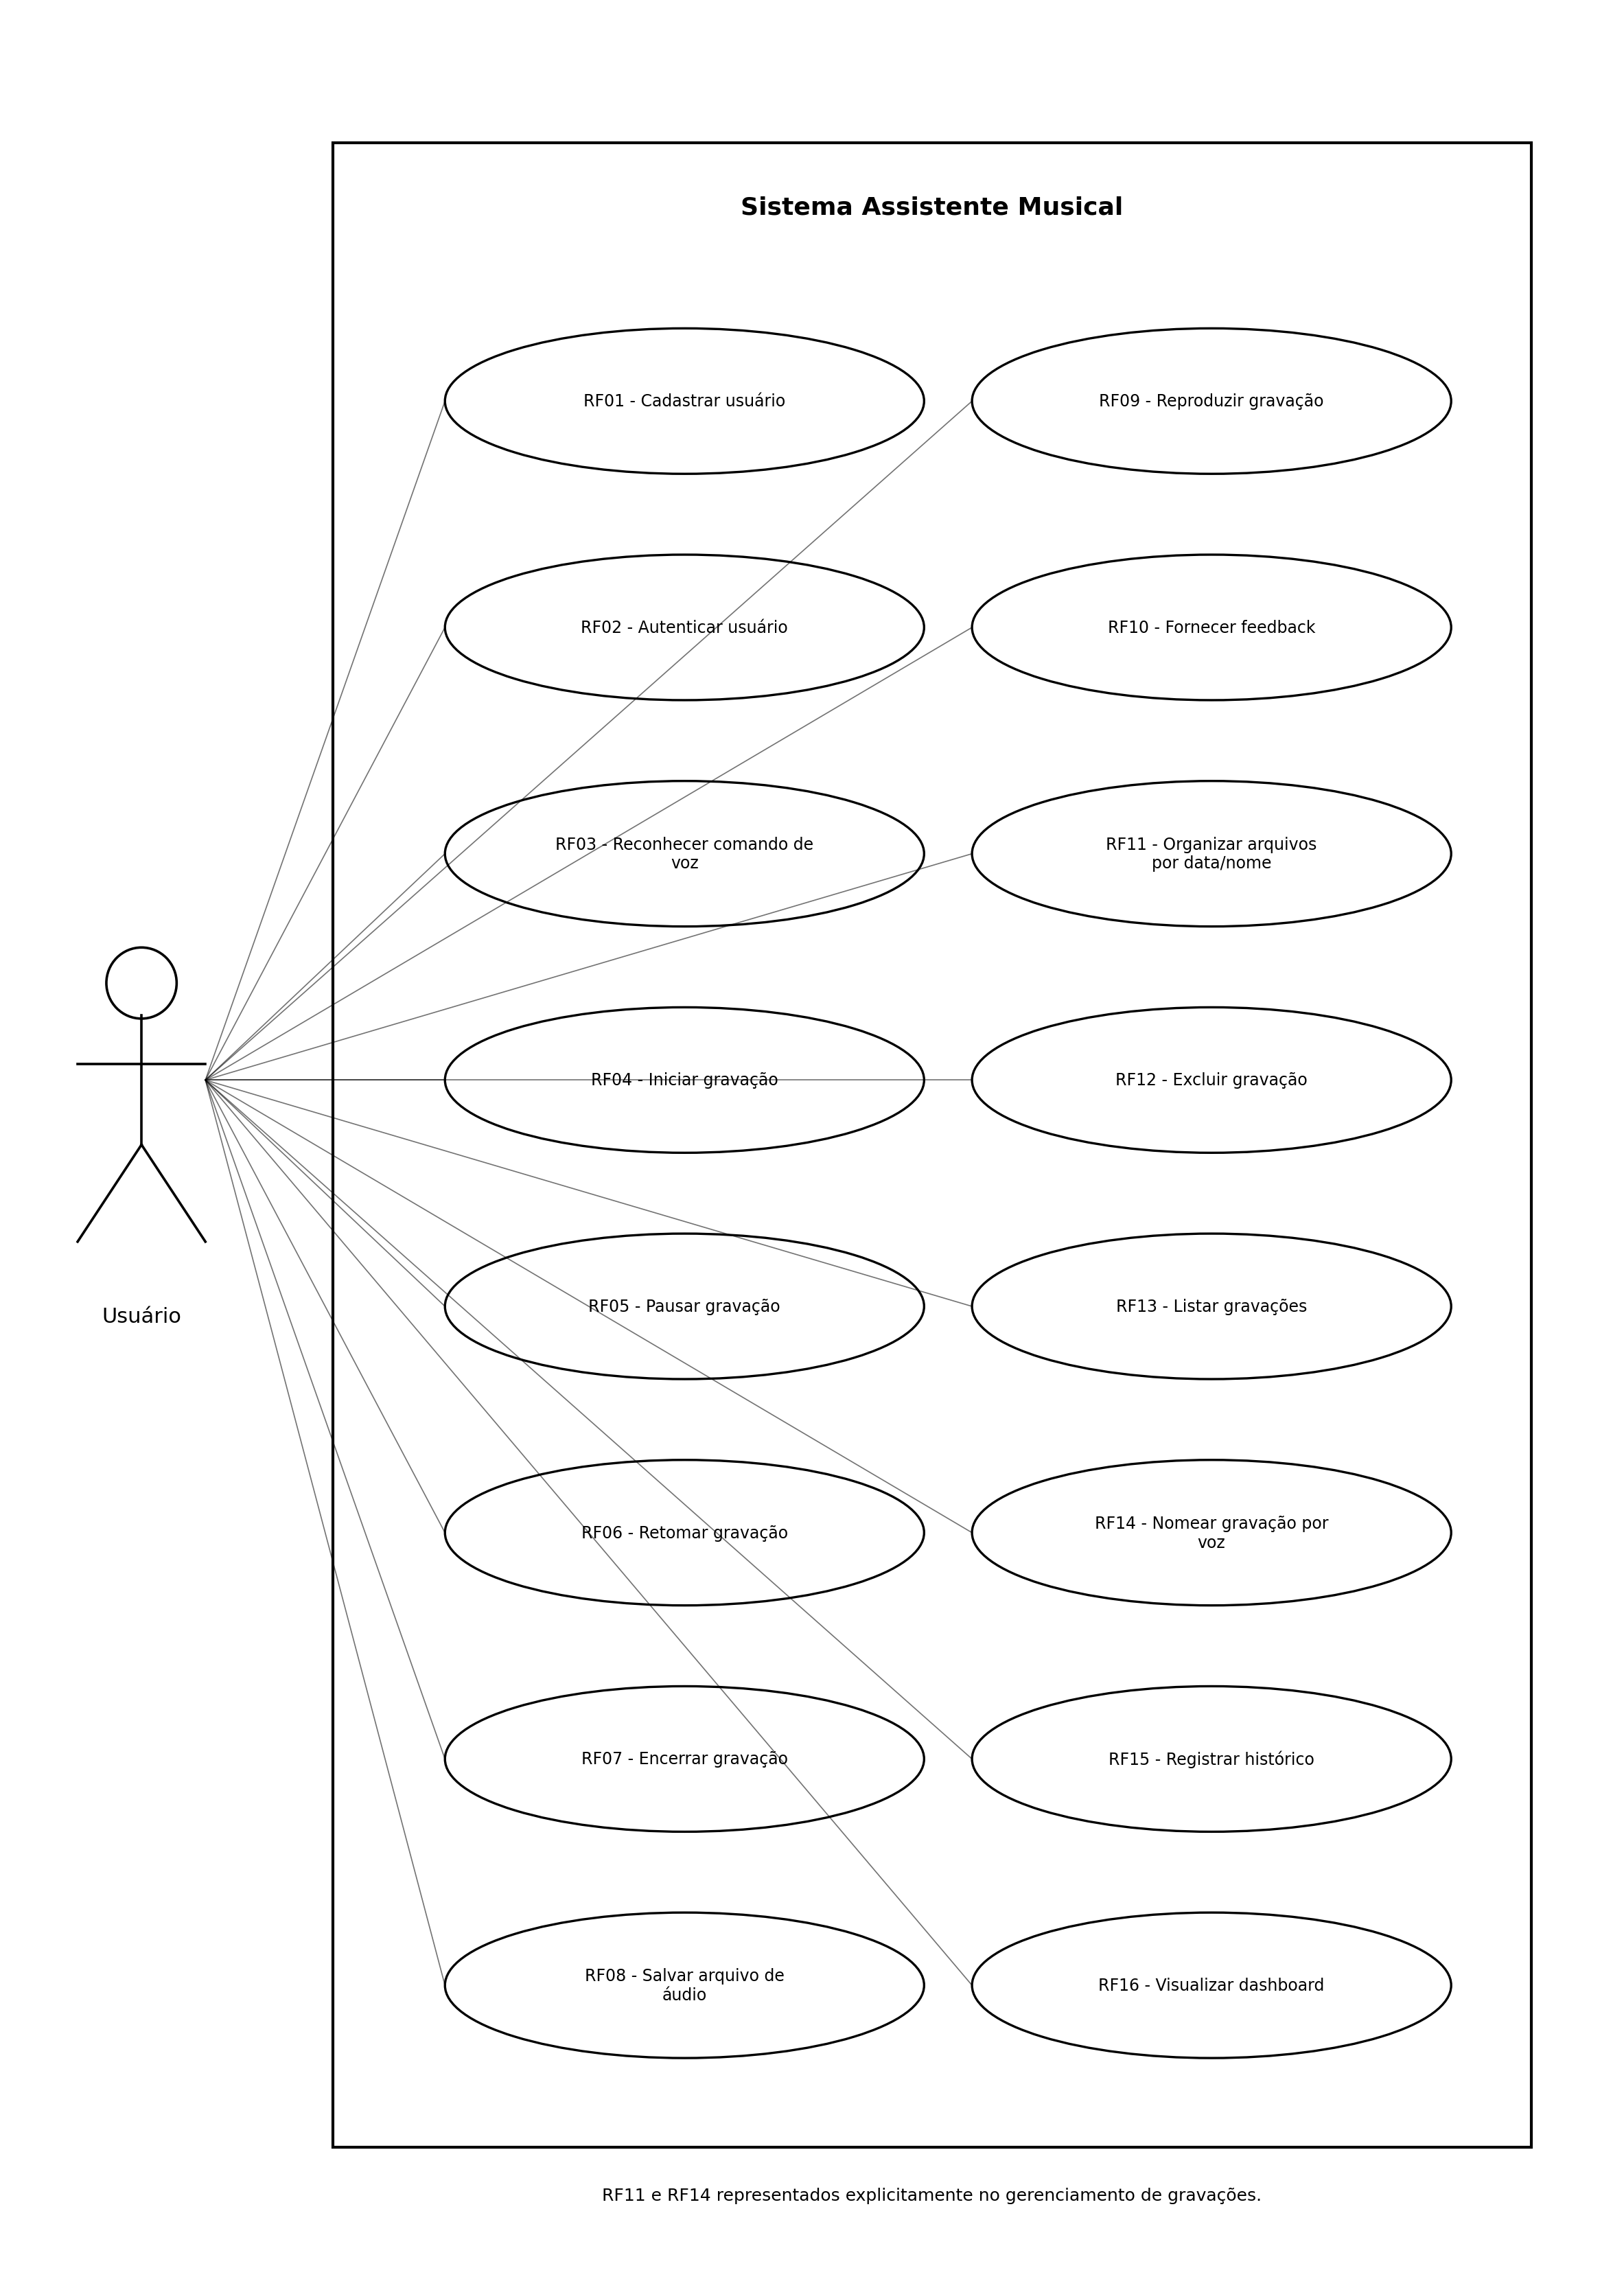
\includegraphics[height=0.97\textheight,keepaspectratio]{diagrama-caso-uso-assistente.png}

\fontefigura{Autoria própria.}

\label{fig:caso-uso-assistente}

\end{figure}



\section{ESPECIFICAÇÃO DOS CASOS DE USO}



A especificação dos casos de uso descreve detalhadamente o comportamento do sistema em relação às interações do usuário. Para atender aos requisitos definidos, foi elaborada uma especificação para cada requisito funcional do sistema, contendo ator, descrição, pré-condição, pós-condição, fluxo principal, fluxo alternativo e fluxo de erro.



\clearpage
\subsection*{RF01 -- CASO DE USO: CADASTRAR USUÁRIO}



\textbf{Ator:} Usuário.



\textbf{Descrição:} Permite que o usuário realize seu cadastro no sistema.



\textbf{Pré-condição:} O usuário deve estar na tela de cadastro.



\textbf{Pós-condição:} Os dados do usuário são armazenados no banco de dados.



\textbf{Fluxo principal:}

\begin{enumerate}

    \item O usuário acessa a tela de cadastro.

    \item O usuário informa nome, e-mail e senha.

    \item O sistema valida os dados informados.

    \item O sistema armazena os dados no banco de dados.

    \item O sistema informa que o cadastro foi realizado com sucesso.

\end{enumerate}



\textbf{Fluxo alternativo:}

\begin{enumerate}

    \item Caso o usuário já possua cadastro, o sistema permite retornar para a tela de login.

\end{enumerate}



\textbf{Fluxo de erro:}

\begin{enumerate}

    \item Caso algum campo obrigatório esteja vazio, o sistema solicita o preenchimento.

    \item Caso o e-mail já esteja cadastrado, o sistema informa que não é possível concluir o cadastro.

\end{enumerate}



\clearpage
\subsection*{RF02 -- CASO DE USO: AUTENTICAR USUÁRIO}



\textbf{Ator:} Usuário.



\textbf{Descrição:} Permite que o usuário acesse o sistema por meio de e-mail e senha.



\textbf{Pré-condição:} O usuário deve estar cadastrado no sistema.



\textbf{Pós-condição:} O usuário é direcionado para a tela inicial do sistema.



\textbf{Fluxo principal:}

\begin{enumerate}

    \item O usuário acessa a tela de login.

    \item O usuário informa e-mail e senha.

    \item O sistema valida as credenciais informadas.

    \item O sistema libera o acesso à tela inicial.

\end{enumerate}



\textbf{Fluxo alternativo:}

\begin{enumerate}

    \item Caso o usuário não possua cadastro, o sistema permite acessar a tela de cadastro.

\end{enumerate}



\textbf{Fluxo de erro:}

\begin{enumerate}

    \item Caso o e-mail ou a senha estejam incorretos, o sistema exibe uma mensagem de erro.

\end{enumerate}



\clearpage
\subsection*{RF03 -- CASO DE USO: RECONHECER COMANDO DE VOZ}



\textbf{Ator:} Usuário.



\textbf{Descrição:} Permite que o sistema capture e interprete comandos de voz emitidos pelo usuário.



\textbf{Pré-condição:} O usuário deve estar autenticado e o sistema deve ter permissão de acesso ao microfone.



\textbf{Pós-condição:} O comando é interpretado e direcionado para a funcionalidade correspondente.



\textbf{Fluxo principal:}

\begin{enumerate}

    \item O usuário aciona o assistente virtual.

    \item O sistema ativa o reconhecimento de voz.

    \item O usuário emite um comando.

    \item O sistema captura o áudio.

    \item O sistema interpreta o comando.

    \item O sistema identifica a ação correspondente.

\end{enumerate}



\textbf{Fluxo alternativo:}

\begin{enumerate}

    \item Caso o comando seja reconhecido parcialmente, o sistema solicita confirmação do usuário.

\end{enumerate}



\textbf{Fluxo de erro:}

\begin{enumerate}

    \item Caso o comando não seja compreendido, o sistema informa que não conseguiu entender.

    \item O sistema solicita que o usuário repita o comando.

\end{enumerate}



\clearpage
\subsection*{RF04 -- CASO DE USO: INICIAR GRAVAÇÃO}



\textbf{Ator:} Usuário.



\textbf{Descrição:} Permite ao usuário iniciar uma gravação de áudio por meio de comando de voz.



\textbf{Pré-condição:} O usuário deve estar autenticado, o microfone deve estar disponível e não deve existir gravação em andamento.



\textbf{Pós-condição:} A gravação é iniciada e registrada no sistema.



\textbf{Fluxo principal:}

\begin{enumerate}

    \item O usuário emite o comando para iniciar uma gravação.

    \item O sistema reconhece o comando.

    \item O sistema inicia a captura de áudio.

    \item O sistema cria um registro inicial da gravação.

    \item O sistema informa que a gravação foi iniciada.

\end{enumerate}



\textbf{Fluxo alternativo:}

\begin{enumerate}

    \item Caso já exista uma gravação em andamento, o sistema informa que não é possível iniciar outra gravação simultaneamente.

\end{enumerate}



\textbf{Fluxo de erro:}

\begin{enumerate}

    \item Caso o comando não seja compreendido, o sistema solicita repetição.

    \item Caso o microfone não esteja disponível, o sistema exibe uma mensagem de erro.

\end{enumerate}



\clearpage
\subsection*{RF05 -- CASO DE USO: PAUSAR GRAVAÇÃO}



\textbf{Ator:} Usuário.



\textbf{Descrição:} Permite pausar uma gravação em andamento.



\textbf{Pré-condição:} Deve existir uma gravação ativa.



\textbf{Pós-condição:} A gravação fica com status pausado.



\textbf{Fluxo principal:}

\begin{enumerate}

    \item O usuário emite o comando para pausar a gravação.

    \item O sistema reconhece o comando.

    \item O sistema pausa a captura de áudio.

    \item O sistema atualiza o status da gravação para pausada.

    \item O sistema informa que a gravação foi pausada.

\end{enumerate}



\textbf{Fluxo alternativo:}

\begin{enumerate}

    \item Caso não exista gravação em andamento, o sistema informa que não há gravação ativa.

\end{enumerate}



\textbf{Fluxo de erro:}

\begin{enumerate}

    \item Caso o comando não seja compreendido, o sistema solicita repetição.

\end{enumerate}



\clearpage
\subsection*{RF06 -- CASO DE USO: RETOMAR GRAVAÇÃO}



\textbf{Ator:} Usuário.



\textbf{Descrição:} Permite retomar uma gravação pausada.



\textbf{Pré-condição:} Deve existir uma gravação pausada.



\textbf{Pós-condição:} A gravação volta ao status em andamento.



\textbf{Fluxo principal:}

\begin{enumerate}

    \item O usuário emite o comando para retomar a gravação.

    \item O sistema reconhece o comando.

    \item O sistema retoma a captura de áudio.

    \item O sistema atualiza o status da gravação.

    \item O sistema informa que a gravação foi retomada.

\end{enumerate}



\textbf{Fluxo alternativo:}

\begin{enumerate}

    \item Caso não exista gravação pausada, o sistema informa que não há gravação para retomar.

\end{enumerate}



\textbf{Fluxo de erro:}

\begin{enumerate}

    \item Caso o comando não seja compreendido, o sistema solicita repetição.

\end{enumerate}



\clearpage
\subsection*{RF07 -- CASO DE USO: ENCERRAR GRAVAÇÃO}



\textbf{Ator:} Usuário.



\textbf{Descrição:} Permite encerrar uma gravação em andamento ou pausada.



\textbf{Pré-condição:} Deve existir uma gravação em andamento ou pausada.



\textbf{Pós-condição:} A gravação é finalizada.



\textbf{Fluxo principal:}

\begin{enumerate}

    \item O usuário emite o comando para encerrar a gravação.

    \item O sistema reconhece o comando.

    \item O sistema finaliza a captura de áudio.

    \item O sistema altera o status da gravação para finalizada.

    \item O sistema informa que a gravação foi encerrada.

\end{enumerate}



\textbf{Fluxo alternativo:}

\begin{enumerate}

    \item Caso a gravação esteja pausada, o sistema encerra a gravação a partir do estado pausado.

\end{enumerate}



\textbf{Fluxo de erro:}

\begin{enumerate}

    \item Caso não exista gravação ativa ou pausada, o sistema informa que não há gravação para encerrar.

\end{enumerate}



\clearpage
\subsection*{RF08 -- CASO DE USO: SALVAR ARQUIVO DE ÁUDIO}



\textbf{Ator:} Usuário.



\textbf{Descrição:} Permite que o sistema salve automaticamente o arquivo de áudio após a finalização da gravação.



\textbf{Pré-condição:} A gravação deve ter sido encerrada corretamente.



\textbf{Pós-condição:} O arquivo de áudio é salvo no armazenamento local e registrado no banco de dados.



\textbf{Fluxo principal:}

\begin{enumerate}

    \item O sistema recebe a solicitação de salvamento após o encerramento da gravação.

    \item O sistema gera o arquivo de áudio.

    \item O sistema define o caminho de armazenamento local.

    \item O sistema salva o arquivo.

    \item O sistema registra os dados do arquivo no banco de dados.

\end{enumerate}



\textbf{Fluxo alternativo:}

\begin{enumerate}

    \item Caso o usuário não informe um nome, o sistema salva o arquivo com um nome automático baseado na data e hora.

\end{enumerate}



\textbf{Fluxo de erro:}

\begin{enumerate}

    \item Caso ocorra erro no armazenamento, o sistema informa que não foi possível salvar a gravação.

\end{enumerate}



\clearpage
\subsection*{RF09 -- CASO DE USO: REPRODUZIR GRAVAÇÃO}



\textbf{Ator:} Usuário.



\textbf{Descrição:} Permite reproduzir uma gravação salva.



\textbf{Pré-condição:} Deve existir pelo menos uma gravação salva.



\textbf{Pós-condição:} A gravação selecionada é reproduzida.



\textbf{Fluxo principal:}

\begin{enumerate}

    \item O usuário acessa a lista de gravações.

    \item O usuário seleciona uma gravação.

    \item O sistema localiza o arquivo de áudio.

    \item O sistema inicia a reprodução.

    \item O sistema registra a ação no histórico.

\end{enumerate}



\textbf{Fluxo alternativo:}

\begin{enumerate}

    \item Caso não existam gravações, o sistema informa que nenhuma gravação foi encontrada.

\end{enumerate}



\textbf{Fluxo de erro:}

\begin{enumerate}

    \item Caso o arquivo não seja encontrado, o sistema informa erro ao usuário.

\end{enumerate}



\clearpage
\subsection*{RF10 -- CASO DE USO: FORNECER FEEDBACK AO USUÁRIO}



\textbf{Ator:} Usuário.



\textbf{Descrição:} Permite que o sistema forneça feedback visual e/ou auditivo após a execução de comandos ou ocorrência de erros.



\textbf{Pré-condição:} O usuário deve executar uma ação no sistema.



\textbf{Pós-condição:} O usuário recebe uma confirmação ou aviso sobre a ação executada.



\textbf{Fluxo principal:}

\begin{enumerate}

    \item O usuário executa uma ação por comando de voz ou pela interface.

    \item O sistema processa a ação.

    \item O sistema gera uma mensagem de retorno.

    \item O sistema apresenta feedback visual e/ou auditivo ao usuário.

\end{enumerate}



\textbf{Fluxo alternativo:}

\begin{enumerate}

    \item Caso o feedback auditivo não esteja disponível, o sistema apresenta apenas feedback visual.

\end{enumerate}



\textbf{Fluxo de erro:}

\begin{enumerate}

    \item Caso ocorra falha na emissão do feedback, o sistema registra a falha internamente.

\end{enumerate}



\clearpage
\subsection*{RF11 -- CASO DE USO: ORGANIZAR ARQUIVOS}



\textbf{Ator:} Usuário.



\textbf{Descrição:} Permite organizar os arquivos de áudio por data ou nome.



\textbf{Pré-condição:} Deve existir pelo menos uma gravação salva.



\textbf{Pós-condição:} As gravações são exibidas conforme o critério de organização selecionado.



\textbf{Fluxo principal:}

\begin{enumerate}

    \item O usuário acessa a tela de gravações.

    \item O usuário seleciona o critério de organização.

    \item O sistema consulta as gravações salvas.

    \item O sistema ordena os arquivos por data ou nome.

    \item O sistema exibe a lista organizada.

\end{enumerate}



\textbf{Fluxo alternativo:}

\begin{enumerate}

    \item Caso o usuário não selecione um critério, o sistema utiliza a organização padrão por data.

\end{enumerate}



\textbf{Fluxo de erro:}

\begin{enumerate}

    \item Caso ocorra falha na consulta dos dados, o sistema informa que não foi possível organizar os arquivos.

\end{enumerate}



\clearpage
\subsection*{RF12 -- CASO DE USO: EXCLUIR GRAVAÇÃO}



\textbf{Ator:} Usuário.



\textbf{Descrição:} Permite excluir uma gravação salva no sistema.



\textbf{Pré-condição:} Deve existir pelo menos uma gravação cadastrada.



\textbf{Pós-condição:} A gravação é removida do sistema.



\textbf{Fluxo principal:}

\begin{enumerate}

    \item O usuário acessa a lista de gravações.

    \item O usuário seleciona a gravação desejada.

    \item O usuário solicita a exclusão.

    \item O sistema remove o arquivo de áudio.

    \item O sistema remove ou atualiza o registro da gravação.

    \item O sistema registra a ação no histórico.

\end{enumerate}



\textbf{Fluxo alternativo:}

\begin{enumerate}

    \item Caso o sistema solicite confirmação, o usuário confirma a exclusão antes da remoção.

\end{enumerate}



\textbf{Fluxo de erro:}

\begin{enumerate}

    \item Caso a gravação não seja encontrada, o sistema informa erro ao usuário.

\end{enumerate}



\clearpage
\subsection*{RF13 -- CASO DE USO: LISTAR GRAVAÇÕES}



\textbf{Ator:} Usuário.



\textbf{Descrição:} Permite listar as gravações existentes no sistema.



\textbf{Pré-condição:} O usuário deve estar autenticado.



\textbf{Pós-condição:} O sistema exibe a lista de gravações cadastradas.



\textbf{Fluxo principal:}

\begin{enumerate}

    \item O usuário acessa a tela de gravações.

    \item O sistema consulta as gravações associadas ao usuário.

    \item O sistema exibe a lista de gravações encontradas.

\end{enumerate}



\textbf{Fluxo alternativo:}

\begin{enumerate}

    \item Caso não existam gravações, o sistema exibe uma mensagem informando que a lista está vazia.

\end{enumerate}



\textbf{Fluxo de erro:}

\begin{enumerate}

    \item Caso ocorra falha na consulta dos dados, o sistema informa que não foi possível listar as gravações.

\end{enumerate}



\clearpage
\subsection*{RF14 -- CASO DE USO: NOMEAR GRAVAÇÃO POR COMANDO DE VOZ}



\textbf{Ator:} Usuário.



\textbf{Descrição:} Permite nomear ou renomear uma gravação por meio de comando de voz.



\textbf{Pré-condição:} Deve existir uma gravação cadastrada ou em processo de finalização.



\textbf{Pós-condição:} A gravação recebe o nome informado pelo usuário.



\textbf{Fluxo principal:}

\begin{enumerate}

    \item O usuário emite o comando para nomear a gravação.

    \item O sistema reconhece o comando.

    \item O sistema identifica o nome informado.

    \item O sistema atualiza o nome da gravação.

    \item O sistema registra a ação no histórico.

\end{enumerate}



\textbf{Fluxo alternativo:}

\begin{enumerate}

    \item Caso o nome seja reconhecido parcialmente, o sistema solicita confirmação do usuário.

\end{enumerate}



\textbf{Fluxo de erro:}

\begin{enumerate}

    \item Caso o nome não seja identificado, o sistema solicita que o usuário repita o comando.

\end{enumerate}



\clearpage
\subsection*{RF15 -- CASO DE USO: REGISTRAR HISTÓRICO DE GRAVAÇÕES}



\textbf{Ator:} Usuário.



\textbf{Descrição:} Permite registrar o histórico de gravações e ações realizadas no sistema.



\textbf{Pré-condição:} O usuário deve executar uma ação relacionada às gravações.



\textbf{Pós-condição:} A ação é registrada no histórico do sistema.



\textbf{Fluxo principal:}

\begin{enumerate}

    \item O usuário executa uma ação no sistema.

    \item O sistema identifica a ação realizada.

    \item O sistema registra a ação com data, hora e descrição.

    \item O sistema associa o registro ao usuário e, quando aplicável, à gravação.

\end{enumerate}



\textbf{Fluxo alternativo:}

\begin{enumerate}

    \item Caso a ação não esteja associada a uma gravação específica, o sistema registra apenas a ação vinculada ao usuário.

\end{enumerate}



\textbf{Fluxo de erro:}

\begin{enumerate}

    \item Caso ocorra falha ao salvar o histórico, o sistema informa que a ação foi executada, mas o histórico não foi registrado.

\end{enumerate}



\clearpage
\subsection*{RF16 -- CASO DE USO: VISUALIZAR DASHBOARD}



\textbf{Ator:} Usuário.



\textbf{Descrição:} Permite visualizar um dashboard com indicadores de uso do sistema.



\textbf{Pré-condição:} O usuário deve estar autenticado.



\textbf{Pós-condição:} O sistema apresenta indicadores consolidados ao usuário.



\textbf{Fluxo principal:}

\begin{enumerate}

    \item O usuário acessa a tela de dashboard.

    \item O sistema consulta os dados de gravações, reproduções, comandos e exclusões.

    \item O sistema calcula os indicadores.

    \item O sistema exibe as informações ao usuário.

\end{enumerate}



\textbf{Fluxo alternativo:}

\begin{enumerate}

    \item Caso ainda não existam dados, o sistema exibe os indicadores zerados.

\end{enumerate}



\textbf{Fluxo de erro:}

\begin{enumerate}

    \item Caso ocorra falha na consulta dos dados, o sistema informa que não foi possível carregar o dashboard.

\end{enumerate}



\clearpage

\section{DIAGRAMA DE CLASSES}



O diagrama de classes representa a estrutura estática do sistema, destacando as principais classes, atributos, métodos e relacionamentos. A modelagem contempla as entidades necessárias para cadastro e autenticação de usuários, reconhecimento de comandos de voz, controle de gravações, armazenamento de arquivos de áudio, registro de histórico, emissão de feedback e visualização de indicadores no dashboard.



A Figura \ref{fig:classes-assistente} apresenta o Diagrama de Classes do Assistente Virtual.



\begin{figure}[H]

\centering

\caption{DIAGRAMA DE CLASSES DO ASSISTENTE VIRTUAL}

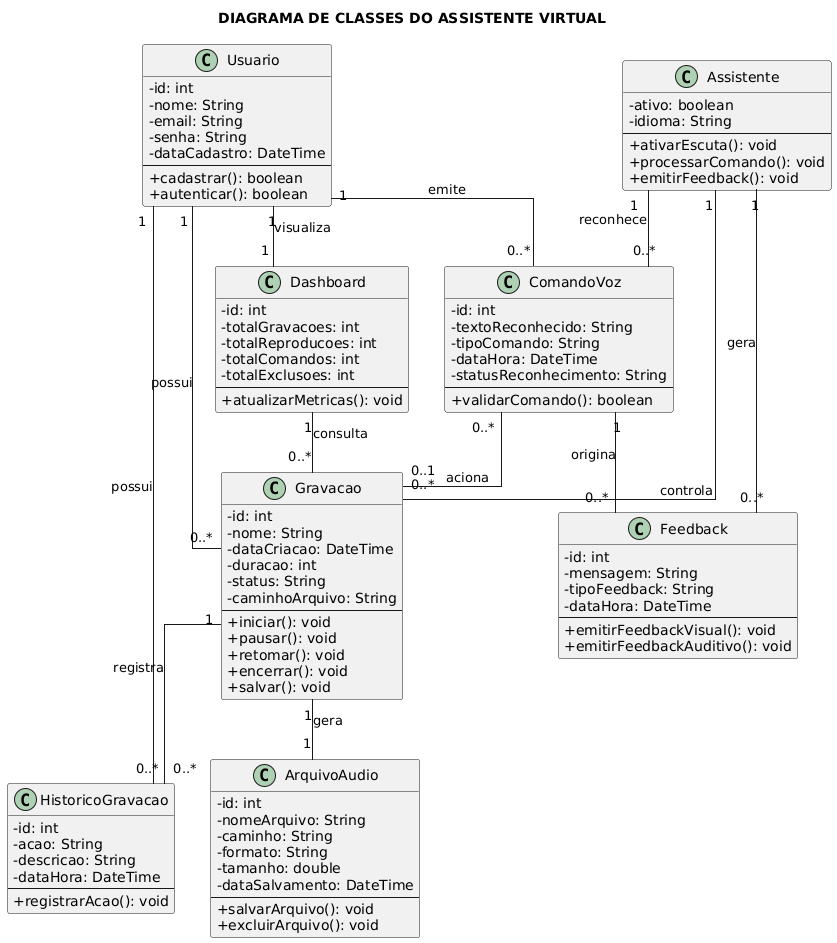
\includegraphics[width=1.07\textwidth,keepaspectratio]{diagrama-classes-assistente.png}

\fontefigura{Autoria própria.}

\label{fig:classes-assistente}

\end{figure}



\clearpage

\section{DIAGRAMA DE SEQUÊNCIA}



O diagrama de sequência demonstra o fluxo de interação entre o usuário e os principais componentes do sistema. A representação contempla o acesso ao sistema, autenticação, ativação do assistente, reconhecimento de comandos de voz, controle de gravações, gerenciamento de gravações, organização de arquivos por data ou nome, nomeação de gravações por comando de voz, consulta ao dashboard e emissão de feedback ao usuário.



A Figura \ref{fig:sequencia-assistente} apresenta o Diagrama de Sequência do Assistente Virtual.



\begin{figure}[H]

\centering

\caption{DIAGRAMA DE SEQUÊNCIA DO ASSISTENTE VIRTUAL}

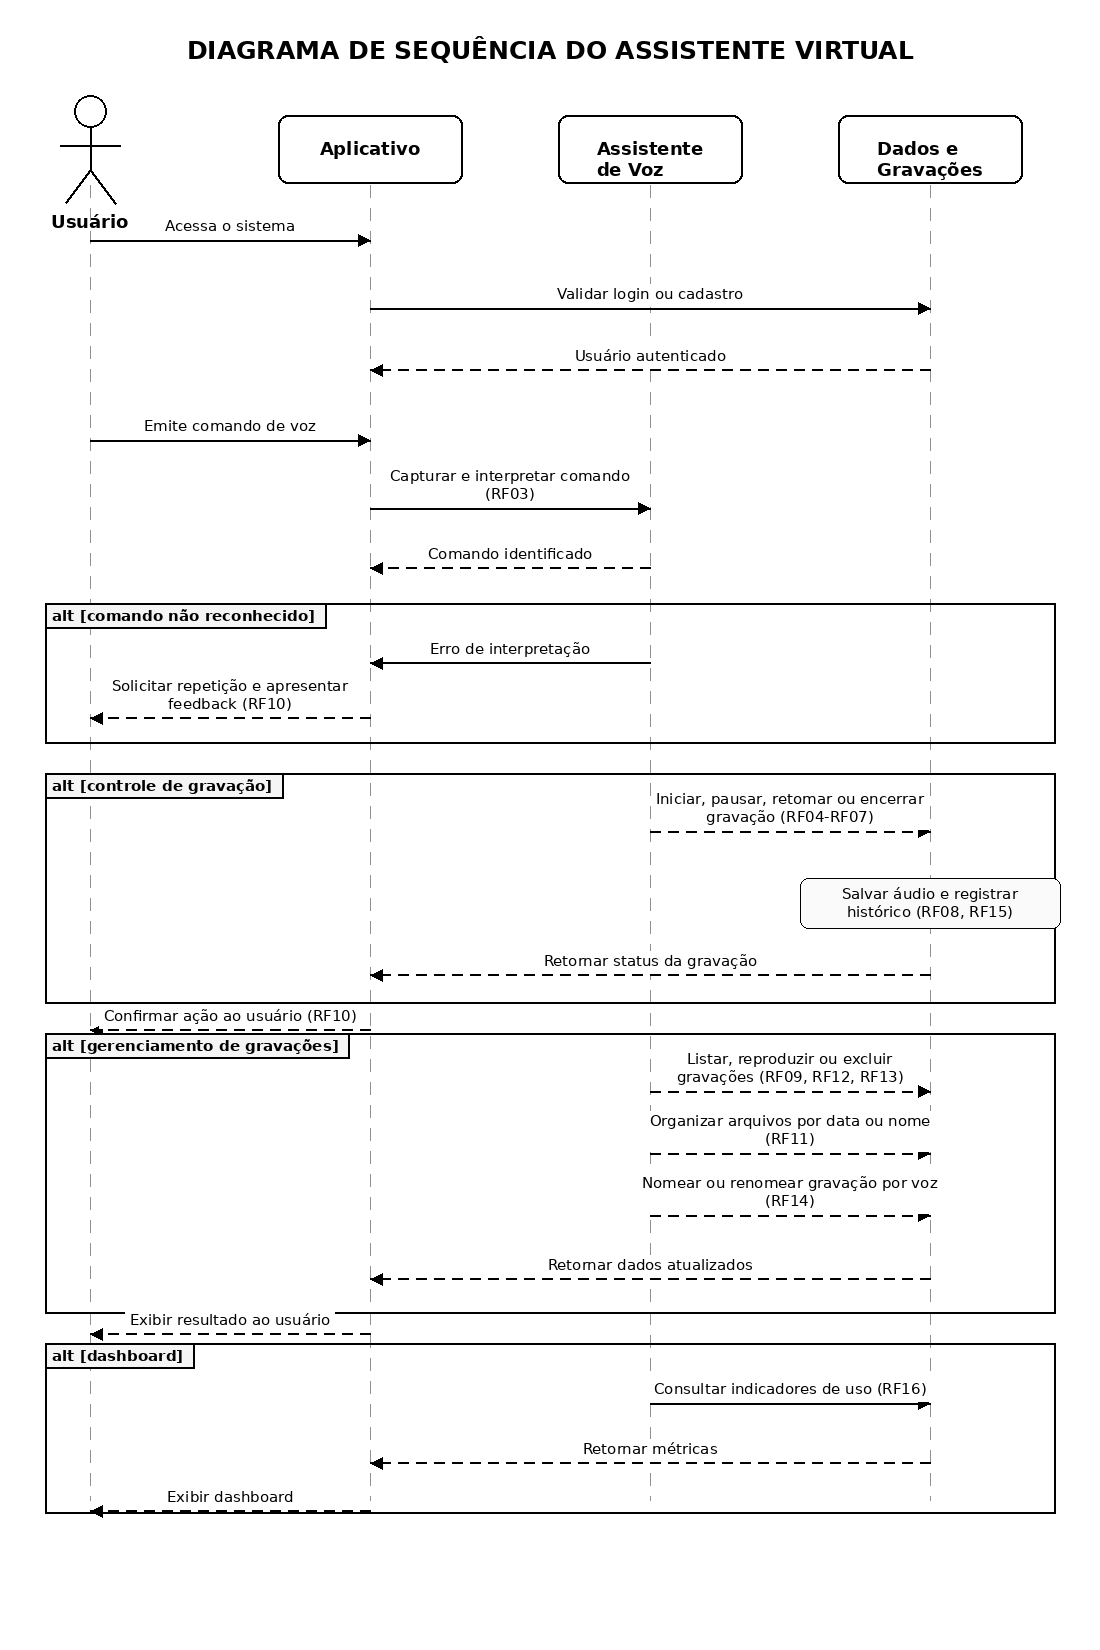
\includegraphics[width=1.07\textwidth,keepaspectratio]{diagrama-sequencia-assistente.png}

\fontefigura{Autoria própria.}

\label{fig:sequencia-assistente}

\end{figure}



\clearpage

\section{DIAGRAMA DE SEQUÊNCIA DE CRIAÇÃO E AUTENTICAÇÃO DE USUÁRIO}



O diagrama de sequência de criação e autenticação de usuário apresenta o fluxo de interação entre o usuário, a interface do sistema, o validador de dados, o banco de dados, a sessão do usuário e o feedback. Esse fluxo contempla o cadastro de um novo usuário, a validação dos dados informados, a verificação de e-mail já cadastrado, o armazenamento das informações e o processo de autenticação para acesso à tela inicial.



A Figura \ref{fig:sequencia-autenticacao} apresenta o Diagrama de Sequência de Criação e Autenticação de Usuário.



\begin{figure}[H]

\centering

\caption{DIAGRAMA DE SEQUÊNCIA DE CRIAÇÃO E AUTENTICAÇÃO DE USUÁRIO}

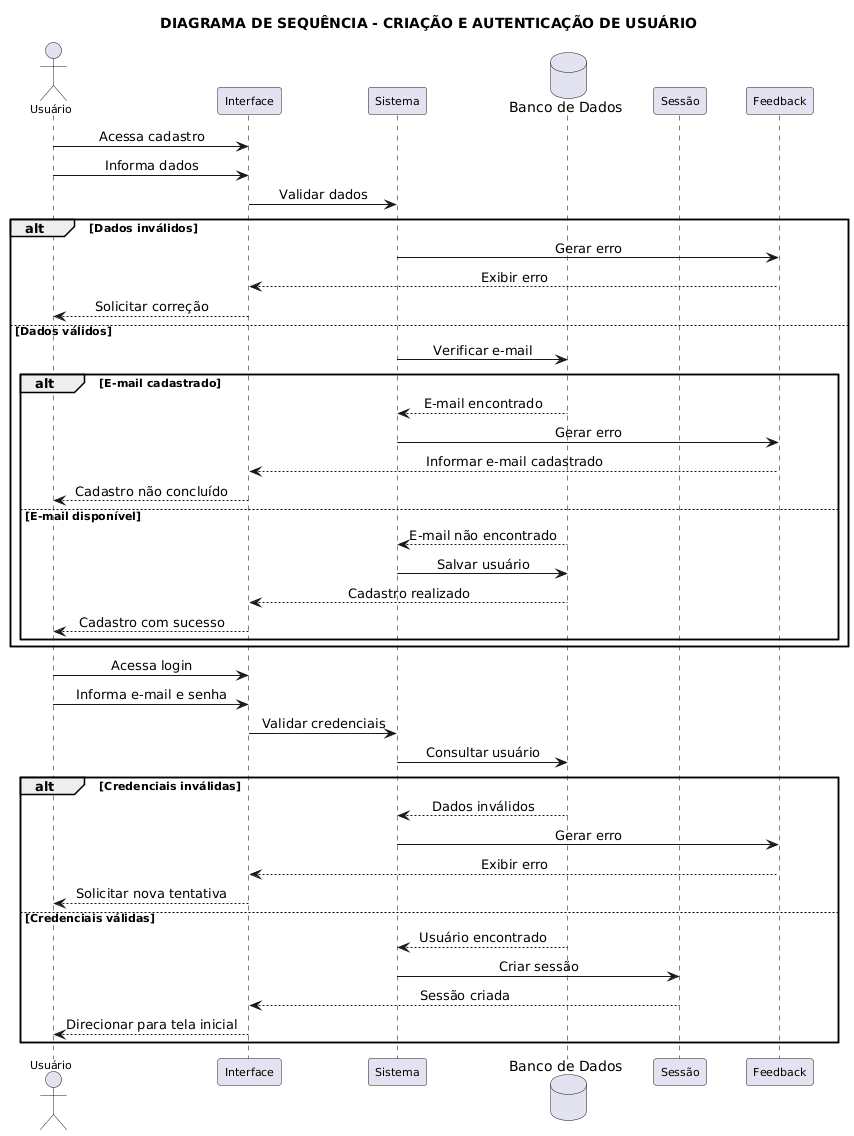
\includegraphics[width=1.08\textwidth,keepaspectratio]{diagrama-sequencia-autenticacao.png}

\fontefigura{Autoria própria.}

\label{fig:sequencia-autenticacao}

\end{figure}



\clearpage

\section{DIAGRAMA DE ARQUITETURA VOICE-FIRST EXPERIMENTAL}



O diagrama de arquitetura voice-first experimental apresenta a organização dos principais componentes relacionados à evolução do assistente virtual para um funcionamento mais orientado por voz. A representação contempla a interface do aplicativo, o gerenciamento centralizado da sessão de voz, o fluxo legado de reconhecimento e gravação, o fluxo experimental de captura em stream, o processamento em isolate, a detecção adaptativa de silêncio, a telemetria e os mecanismos de feedback ao usuário.



Essa arquitetura mantém o fluxo legado como padrão e utiliza recursos experimentais controlados por flags de configuração. Dessa forma, funcionalidades como captura de áudio em stream, processamento em tempo real, detecção de silêncio e roteamento de eventos podem ser avaliadas sem substituir imediatamente os recursos estáveis da aplicação.



A Figura~\ref{fig:arquitetura-voice-first} apresenta o Diagrama de Arquitetura Voice-First Experimental.



\begin{figure}[H]

\centering

\caption{DIAGRAMA DE ARQUITETURA VOICE-FIRST EXPERIMENTAL}

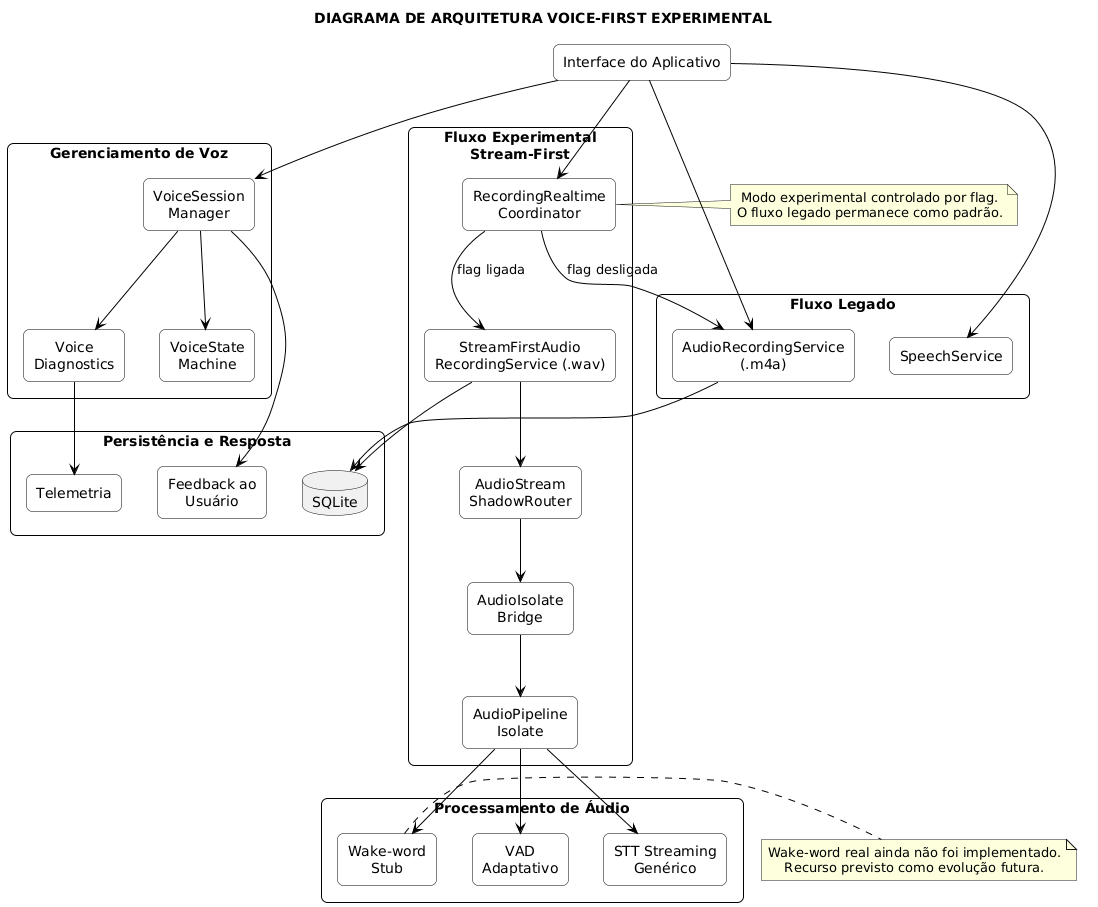
\includegraphics[width=0.95\textwidth,keepaspectratio]{arquitetura-voice-first.png}

\fontefigura{Autoria própria.}

\label{fig:arquitetura-voice-first}

\end{figure}



\clearpage

\section{DIAGRAMA ENTIDADE-RELACIONAMENTO}



O Diagrama Entidade-Relacionamento representa a estrutura lógica do banco de dados do sistema. O modelo contempla as entidades necessárias para armazenar dados de usuário, gravações, arquivos de áudio, comandos de voz, histórico de ações, feedbacks e indicadores do dashboard.



A Figura \ref{fig:der-assistente} apresenta o Diagrama Entidade-Relacionamento do Assistente Virtual.



\begin{figure}[H]

\centering

\caption{DIAGRAMA ENTIDADE-RELACIONAMENTO DO ASSISTENTE VIRTUAL}

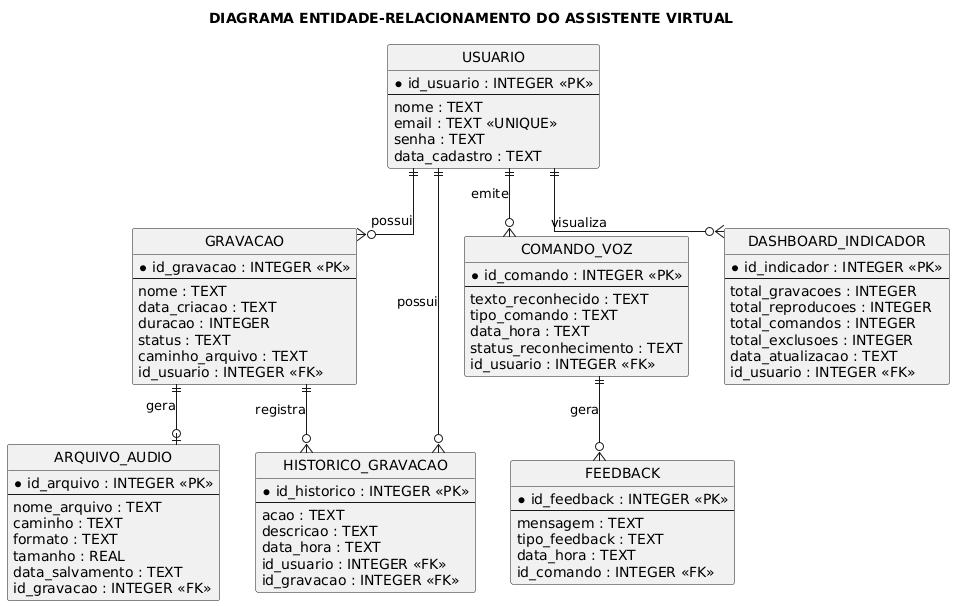
\includegraphics[width=1.07\textwidth,keepaspectratio]{der-assistente.png}

\fontefigura{Autoria própria.}

\label{fig:der-assistente}

\end{figure}



\clearpage

\section{FLUXO DE NAVEGAÇÃO DE TELAS}



O fluxo de navegação de telas apresenta a organização das principais telas do sistema e os caminhos disponíveis ao usuário durante o uso da aplicação. A representação destaca o acesso ao sistema, a tela inicial, o assistente virtual, o gerenciamento de gravações, o histórico, o dashboard, as configurações e o encerramento da sessão.



A Figura~\ref{fig:fluxo} apresenta o fluxo de navegação de telas da aplicação.



\begin{figure}[H]

    \centering

    \caption{FLUXO DE NAVEGAÇÃO DE TELAS}

    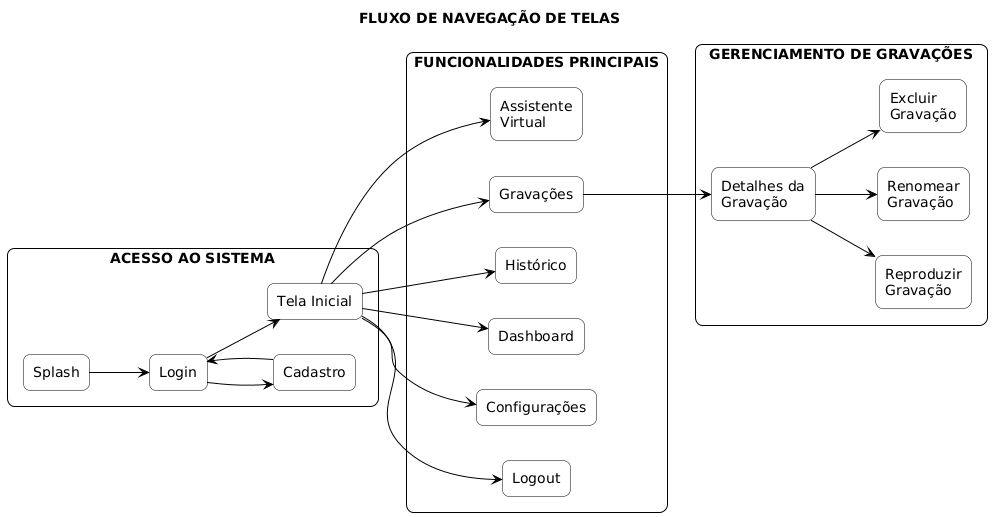
\includegraphics[width=1.05\textwidth,keepaspectratio]{fluxo-navegacao.png}

    \fontefigura{Autoria própria.}

    \label{fig:fluxo}

\end{figure}





% ----------------------------------------------------------

% 7 PROTÓTIPO DO SISTEMA

% ----------------------------------------------------------

\chapter{PROTÓTIPO DO SISTEMA}



Este capítulo apresenta as principais telas do protótipo desenvolvido para o assistente virtual por comando de voz. As telas demonstram a organização da interface, o fluxo de navegação e as funcionalidades previstas para cadastro, autenticação, uso do assistente, gerenciamento de gravações, histórico, dashboard e configurações.



\section{TELA DE LOGIN}



A tela de login permite que o usuário acesse o sistema utilizando e-mail e senha previamente cadastrados.



\begin{figure}[H]

\centering

\caption{TELA DE LOGIN}

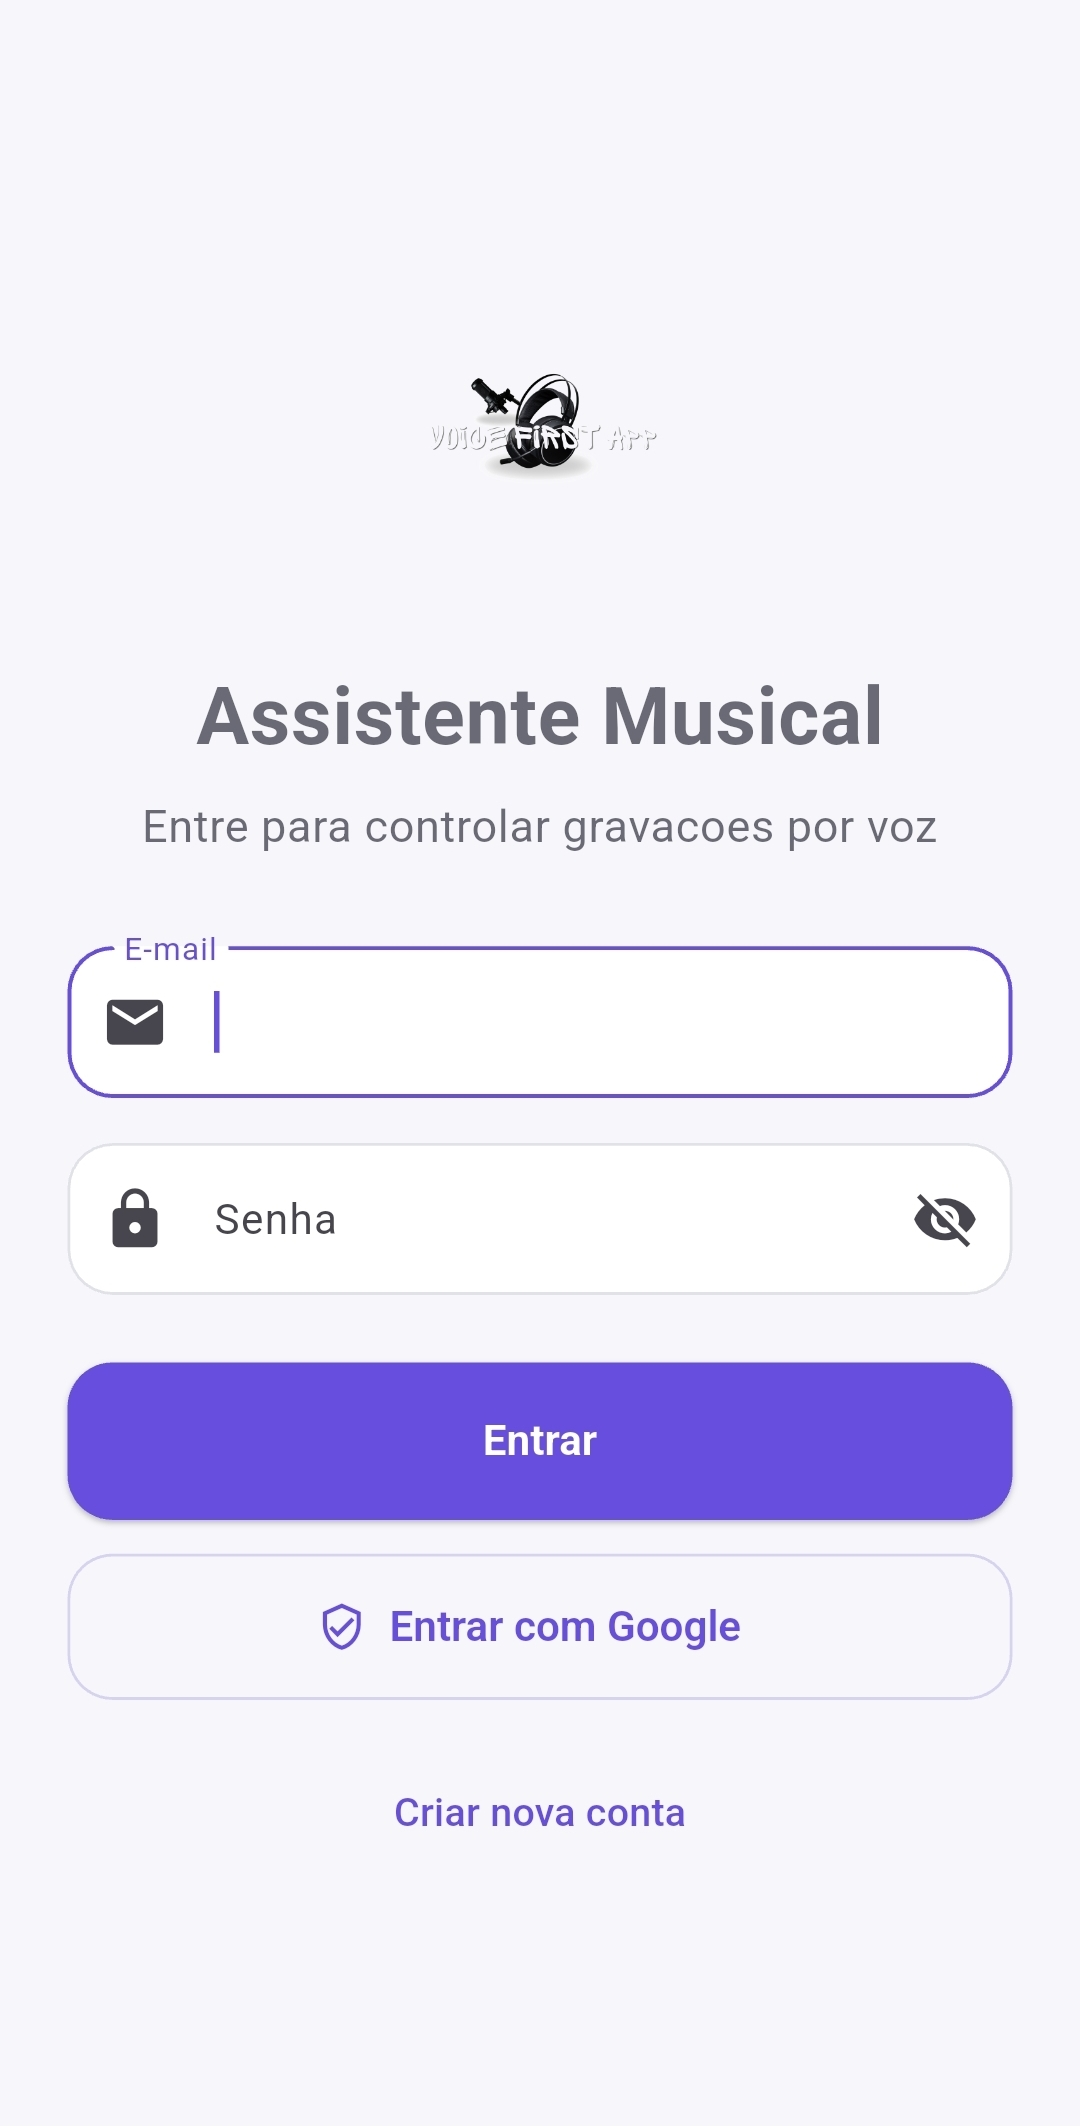
\includegraphics[width=0.45\textwidth,keepaspectratio]{tela-login.jpeg}

\fontefigura{Autoria própria.}

\label{fig:tela-login}

\end{figure}



\section{TELA DE CADASTRO}



A tela de cadastro permite que um novo usuário informe seus dados para criar uma conta no sistema.



\begin{figure}[H]

\centering

\caption{TELA DE CADASTRO}

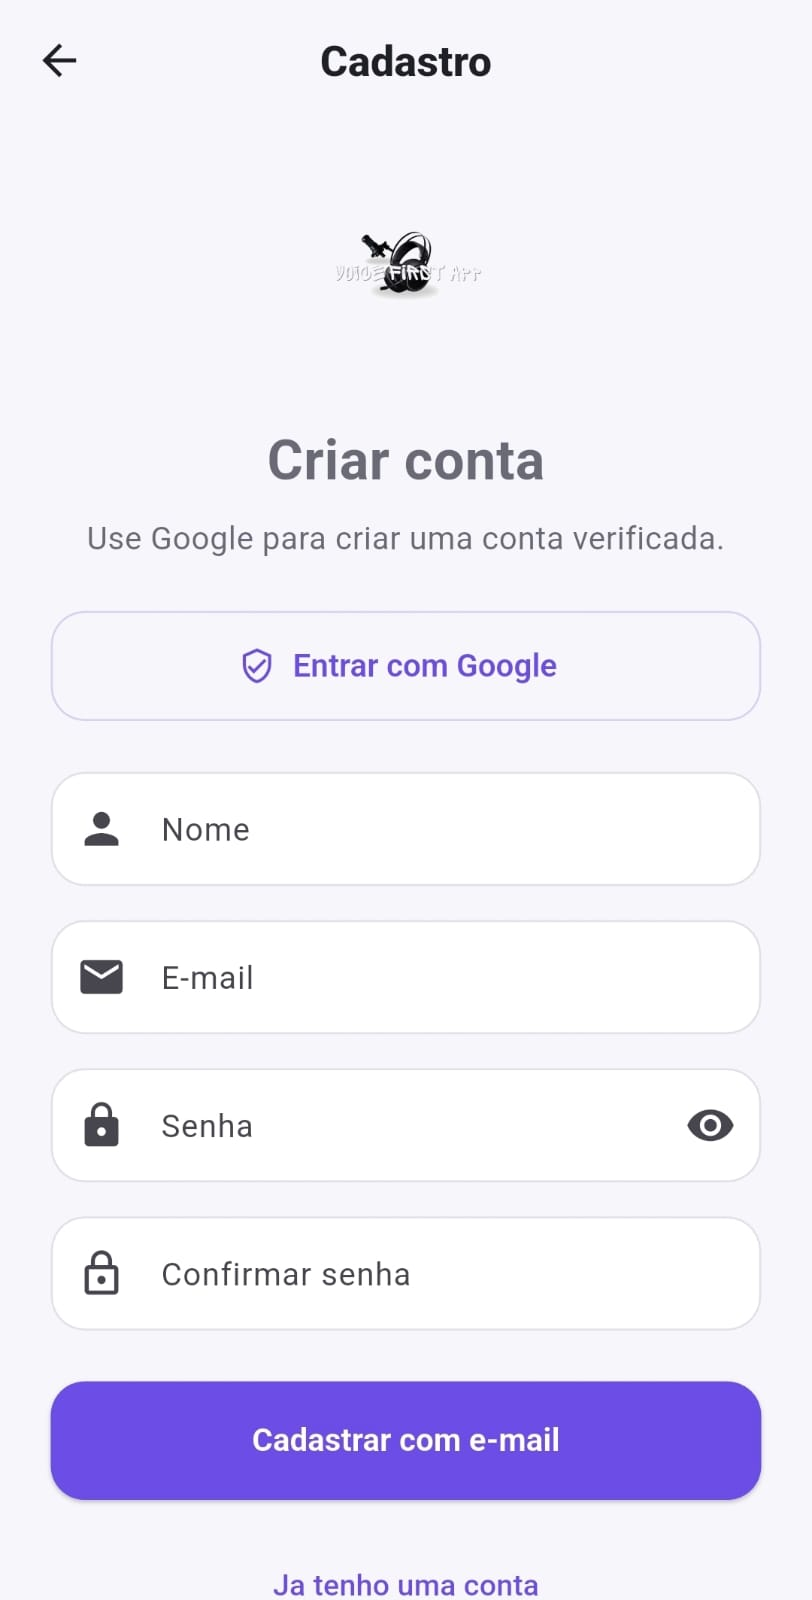
\includegraphics[width=0.57\textwidth,keepaspectratio]{tela-cadastro.jpeg}

\fontefigura{Autoria própria.}

\label{fig:tela-cadastro}

\end{figure}



\section{TELA INICIAL}



A tela inicial reúne os principais acessos do sistema, permitindo ao usuário navegar para as funcionalidades de criação, gravações, histórico, dashboard e configurações. A tela também apresenta o status dos comandos de voz, indicando quando o assistente está disponível para receber instruções.



\begin{figure}[H]

\centering

\caption{TELA INICIAL}

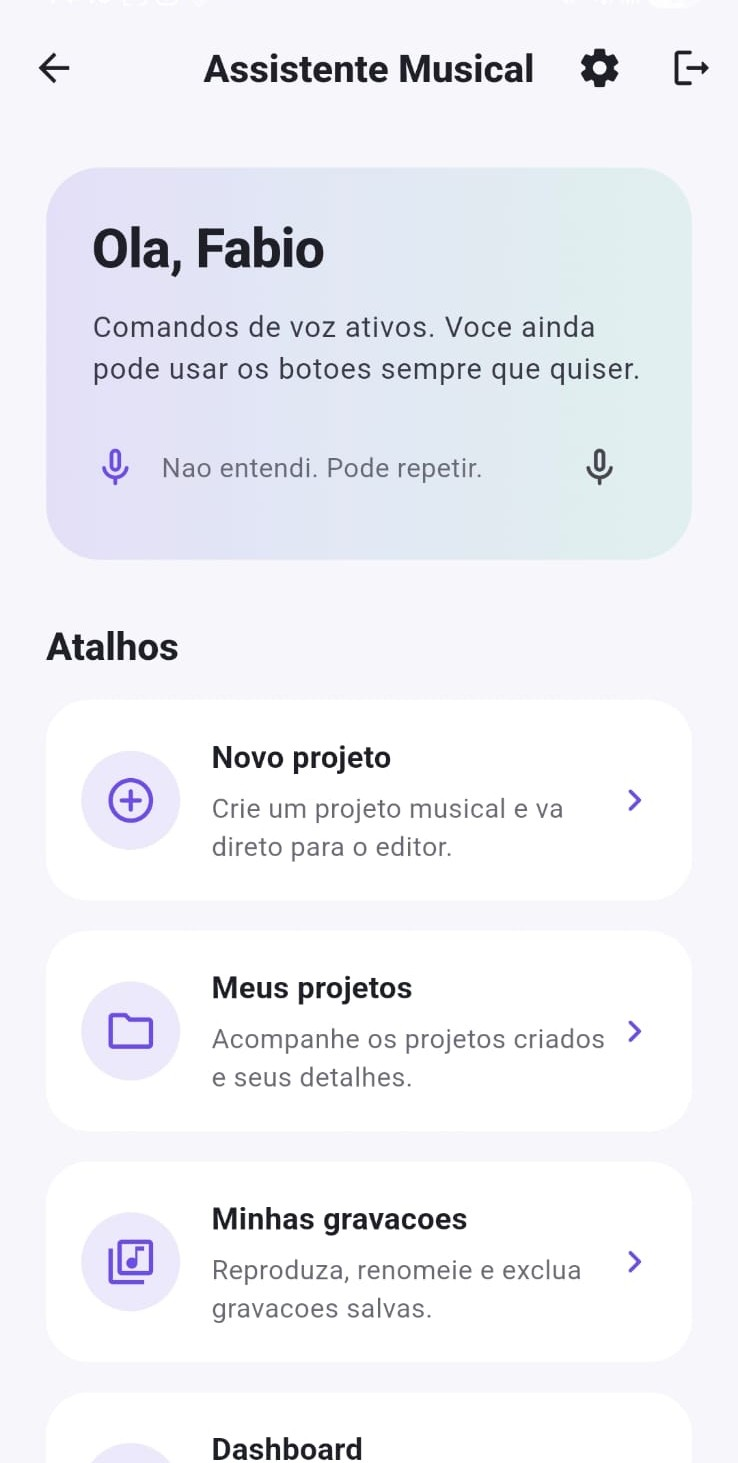
\includegraphics[width=0.57\textwidth,keepaspectratio]{tela-inicial.jpeg}

\fontefigura{Autoria própria.}

\label{fig:tela-inicial}

\end{figure}



\section{TELA DE GRAVAÇÕES}



A tela de gravações apresenta os arquivos de áudio registrados pelo usuário, permitindo buscar, reproduzir e gerenciar gravações salvas.



\begin{figure}[H]

\centering

\caption{TELA DE GRAVAÇÕES}

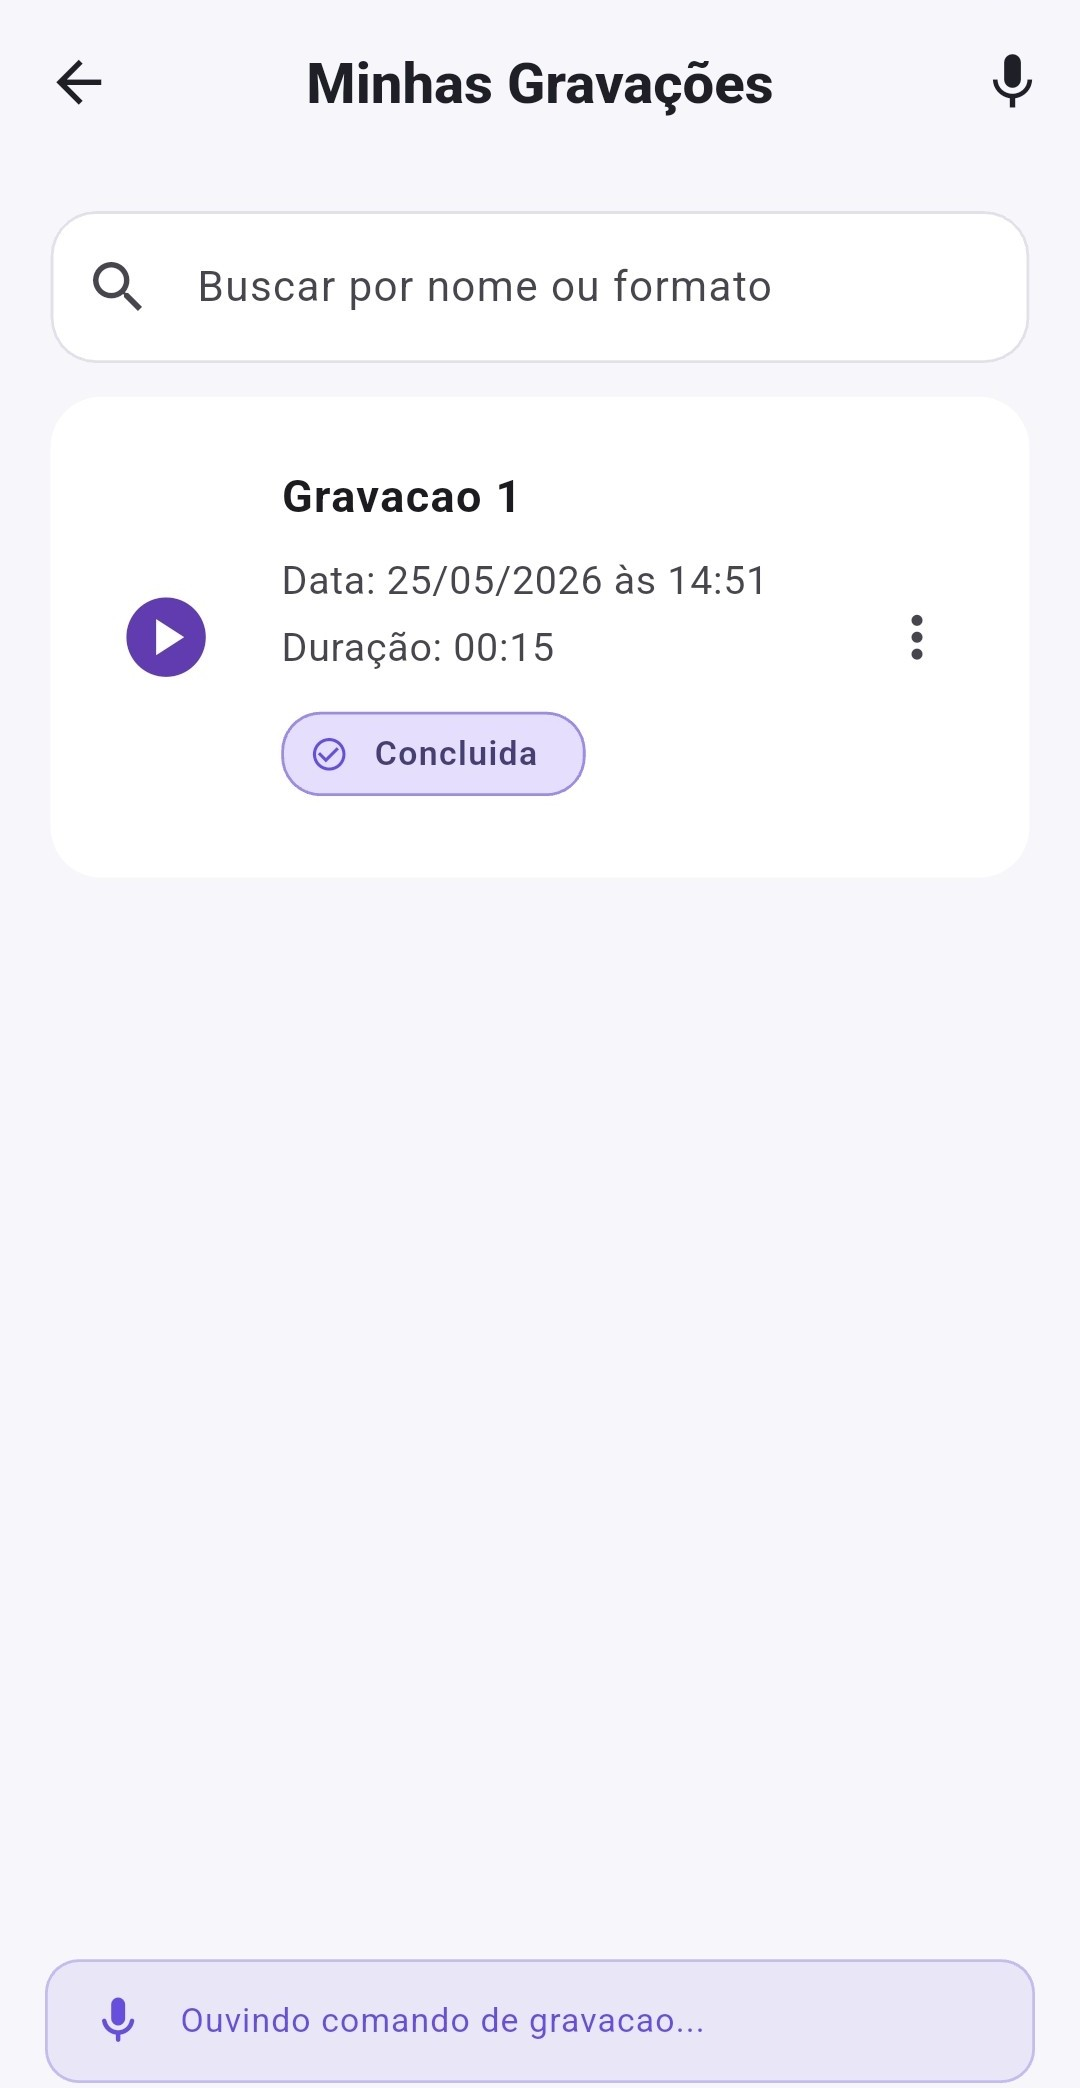
\includegraphics[width=0.57\textwidth,keepaspectratio]{tela-gravacoes.jpeg}

\fontefigura{Autoria própria.}

\label{fig:tela-gravacoes}

\end{figure}



\section{TELA DE HISTÓRICO}



A tela de histórico apresenta os eventos realizados no sistema, como gravações iniciadas e finalizadas. Esse recurso permite acompanhar as ações executadas durante o uso da aplicação.



\begin{figure}[H]

\centering

\caption{TELA DE HISTÓRICO}

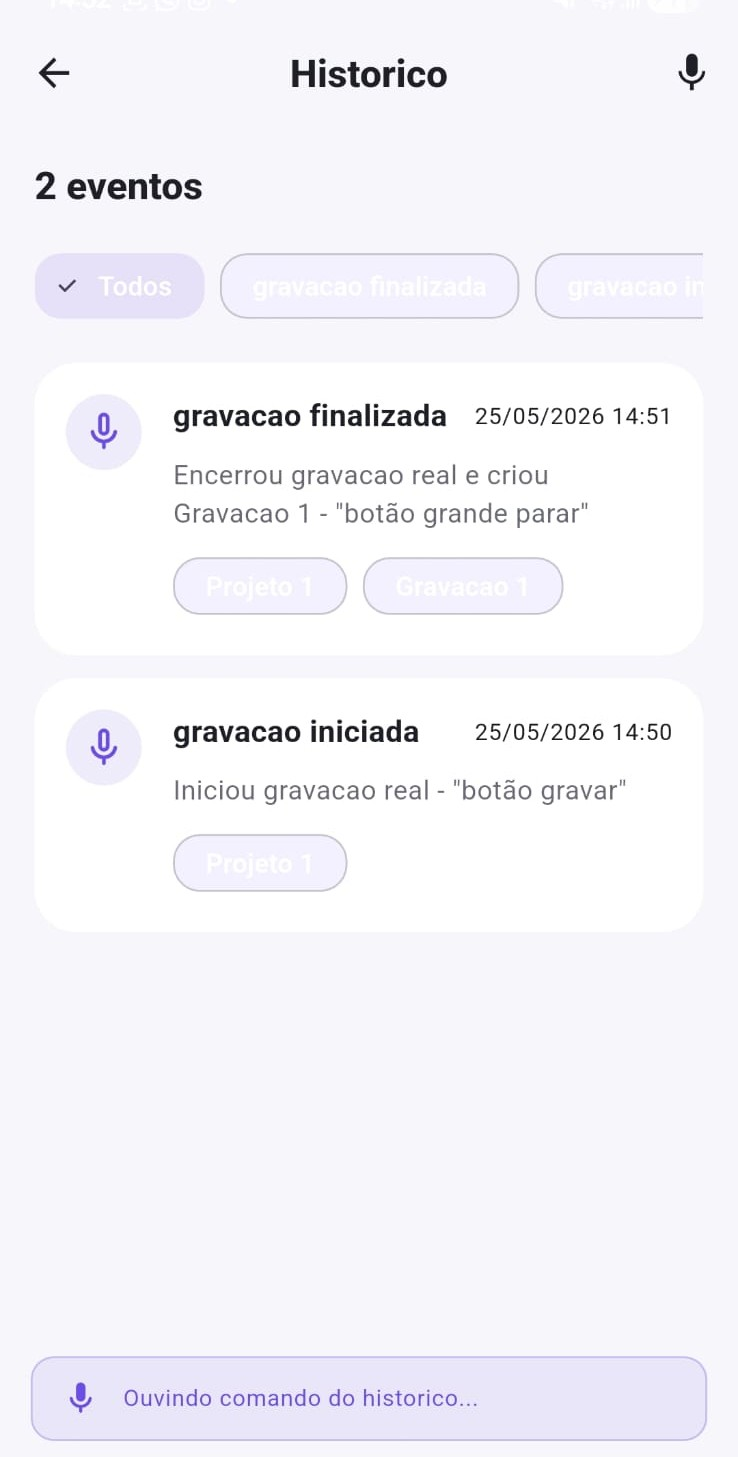
\includegraphics[width=0.57\textwidth,keepaspectratio]{tela-historico.jpeg}

\fontefigura{Autoria própria.}

\label{fig:tela-historico}

\end{figure}



\section{TELA DE DASHBOARD}



A tela de dashboard apresenta indicadores de uso do sistema, como quantidade de projetos, gravações, duração total, comandos reconhecidos, comandos não reconhecidos e eventos recentes.



\begin{figure}[H]

\centering

\caption{TELA DE DASHBOARD}

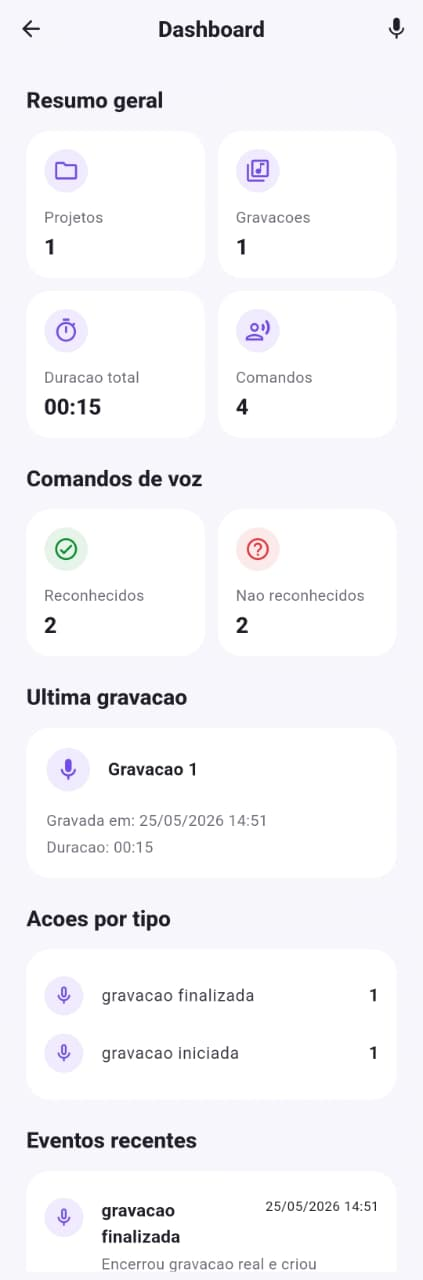
\includegraphics[width=0.4\textwidth,keepaspectratio]{tela-dashboard.jpeg}

\fontefigura{Autoria própria.}

\label{fig:tela-dashboard}

\end{figure}



\section{TELA DE CONFIGURAÇÕES}



A tela de configurações permite consultar ou ajustar preferências da aplicação, incluindo tema visual, controle por voz, escuta contínua, feedback sonoro e comandos personalizados.



\begin{figure}[H]

\centering

\caption{TELA DE CONFIGURAÇÕES}

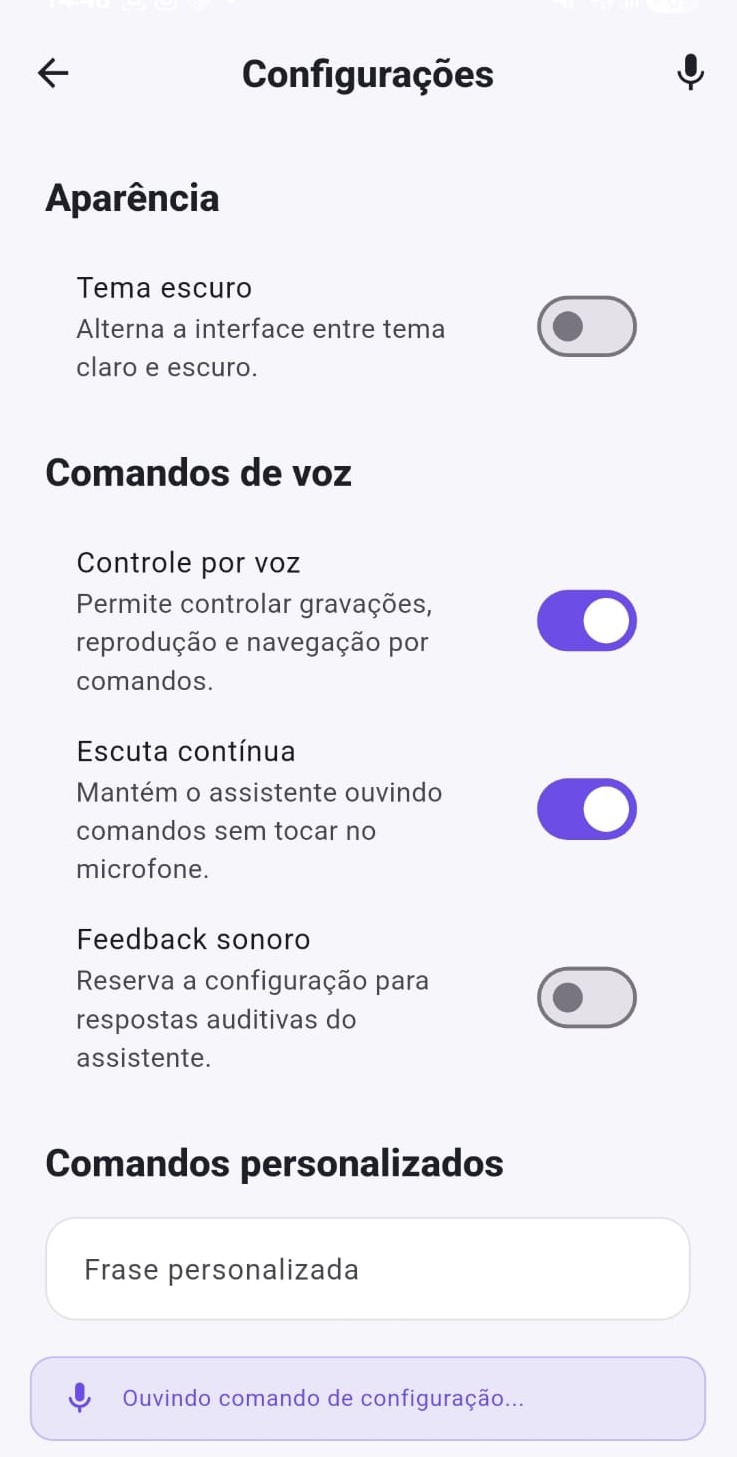
\includegraphics[width=0.57\textwidth,keepaspectratio]{tela-configuracoes.jpeg}

\fontefigura{Autoria própria.}

\label{fig:tela-configuracoes}

\end{figure}



% ----------------------------------------------------------

% 8 MODELAGEM DE DADOS

% ----------------------------------------------------------

\chapter{MODELAGEM DE DADOS}



A modelagem de dados do sistema foi desenvolvida com o objetivo de garantir organização, integridade e eficiência no armazenamento das informações. A estruturação adequada dos dados é fundamental para preservar a consistência das informações e apoiar as funcionalidades previstas no sistema (Sommerville, 2019). O sistema utilizará um banco de dados relacional local, implementado com SQLite, adequado para aplicações móveis que necessitam de funcionamento parcialmente offline.



As principais entidades do sistema são: usuário, gravação, arquivo de áudio, comando de voz, histórico de gravação, feedback e dashboard. A entidade usuário armazena as informações de identificação e acesso, como nome, e-mail, senha e data de cadastro. A entidade gravação registra os dados relacionados aos áudios capturados pelo sistema, como nome, data, duração, status e caminho do arquivo.



A entidade arquivo de áudio armazena informações sobre os arquivos gerados pelas gravações, permitindo registrar nome, caminho, formato, tamanho e data de salvamento. A entidade comando de voz registra os comandos reconhecidos pelo sistema, permitindo acompanhar quais comandos foram emitidos e se foram interpretados corretamente. A entidade histórico de gravação registra ações como iniciar, pausar, retomar, encerrar, reproduzir, organizar, renomear e excluir gravações.



A entidade feedback armazena as mensagens visuais ou auditivas apresentadas ao usuário após ações executadas ou erros identificados. Já a entidade dashboard permite armazenar ou calcular indicadores de uso do sistema, como total de gravações realizadas, gravações reproduzidas, comandos executados e gravações excluídas.



Esse modelo foi projetado para permitir fácil manutenção, integridade dos dados e expansão futura, caso novas funcionalidades sejam adicionadas ao sistema.



% ----------------------------------------------------------

% 9 RELATÓRIO DE TESTES E VALIDAÇÕES

% ----------------------------------------------------------

\chapter{RELATÓRIO DE TESTES E VALIDAÇÕES}



O relatório de testes e validações tem como objetivo apresentar os testes executados no protótipo desenvolvido, verificando se as funcionalidades implementadas atendem aos requisitos definidos para o sistema. Em engenharia de software, a etapa de testes é essencial para identificar falhas, verificar o atendimento aos requisitos e aumentar a confiabilidade do produto desenvolvido (Pressman; Maxim, 2016).

Foram realizados testes funcionais, testes de usabilidade, testes de integração e validações relacionadas à arquitetura voice-first experimental. Os testes contemplaram funcionalidades como cadastro, autenticação, reconhecimento de comandos de voz, controle de gravações, gerenciamento de arquivos, registro de histórico, apresentação de indicadores no dashboard e comportamento do sistema diante de comandos não compreendidos.



\section{CASOS DE TESTE EXECUTADOS}



Os casos de teste executados foram definidos com o objetivo de validar se as funcionalidades do sistema atendem aos requisitos funcionais e não funcionais estabelecidos. Os testes contemplaram cadastro, autenticação, reconhecimento de voz, controle de gravações, gerenciamento de arquivos, histórico, feedback, dashboard e validações específicas da arquitetura voice-first experimental.



\begin{longtable}{|p{1.5cm}|p{2.4cm}|p{5.8cm}|p{4.7cm}|}

\caption{CASOS DE TESTE EXECUTADOS NO SISTEMA}

\label{tab:casos-teste}\\

\hline

\textbf{Caso} & \textbf{Requisito} & \textbf{Objetivo do teste} & \textbf{Resultado esperado} \\

\hline

\endfirsthead



\hline

\textbf{Caso} & \textbf{Requisito} & \textbf{Objetivo do teste} & \textbf{Resultado esperado} \\

\hline

\endhead



CT01 & RF01 & Verificar se o sistema permite cadastrar um novo usuário com nome, e-mail e senha. & Usuário cadastrado com sucesso. \\

\hline

CT02 & RF02 & Verificar se o sistema permite autenticar um usuário com e-mail e senha válidos. & Acesso liberado para a tela inicial. \\

\hline

CT03 & RF03 & Verificar se o sistema reconhece comandos de voz emitidos pelo usuário. & Comando reconhecido e interpretado. \\

\hline

CT04 & RF03 & Verificar o comportamento do sistema quando o comando de voz não for compreendido. & Sistema solicita repetição do comando. \\

\hline

CT05 & RF04 & Verificar se o sistema inicia uma gravação por comando de voz. & Gravação iniciada corretamente. \\

\hline

CT06 & RF05 & Verificar se o sistema pausa uma gravação em andamento. & Gravação pausada. \\

\hline

CT07 & RF06 & Verificar se o sistema retoma uma gravação pausada. & Gravação retomada. \\

\hline

CT08 & RF07 & Verificar se o sistema encerra uma gravação em andamento ou pausada. & Gravação encerrada. \\

\hline

CT09 & RF08 & Verificar se o sistema salva automaticamente o arquivo de áudio após o encerramento da gravação. & Arquivo salvo e registrado no banco de dados. \\

\hline

CT10 & RF09 & Verificar se o sistema reproduz uma gravação salva. & Áudio reproduzido corretamente. \\

\hline

CT11 & RF10 & Verificar se o sistema apresenta feedback visual ou auditivo após uma ação executada. & Feedback apresentado ao usuário. \\

\hline

CT12 & RF11 & Verificar se o sistema organiza os arquivos por data ou nome. & Lista organizada conforme critério selecionado. \\

\hline

CT13 & RF12 & Verificar se o sistema permite excluir uma gravação existente. & Gravação removida do sistema. \\

\hline

CT14 & RF13 & Verificar se o sistema lista as gravações cadastradas. & Lista de gravações exibida. \\

\hline

CT15 & RF14 & Verificar se o sistema permite nomear ou renomear uma gravação por comando de voz. & Nome da gravação atualizado. \\

\hline

CT16 & RF15 & Verificar se o sistema registra ações relacionadas às gravações no histórico. & Histórico atualizado com a ação realizada. \\

\hline

CT17 & RF16 & Verificar se o sistema exibe o dashboard com indicadores de uso. & Indicadores exibidos corretamente. \\

\hline

CT18 & RNF01 & Verificar se comandos simples são respondidos em tempo inferior a 2 segundos. & Tempo de resposta dentro do limite definido. \\

\hline

CT19 & RNF02/\newline RNF09 & Verificar se a interface é simples, intuitiva e fácil de utilizar. & Usuário consegue navegar pelas telas principais sem dificuldade. \\

\hline

CT20 & RNF03 & Verificar se a aplicação é compatível com dispositivos Android versão 8 ou superior. & Aplicação executada em dispositivo compatível. \\

\hline

CT21 & RNF06 & Verificar se o sistema mantém funcionalidades básicas disponíveis parcialmente offline. & Dados locais acessíveis sem conexão constante com a internet. \\

\hline

CT22 & RNF07/\newline RNF10 & Verificar se os dados do usuário, gravações e histórico são armazenados com integridade e segurança. & Dados preservados e associados corretamente ao usuário. \\

\hline

\end{longtable}

\fontetabela{Autoria própria.}


\section{RESULTADOS OBTIDOS NOS TESTES}

Após a execução dos testes, foi possível verificar que as funcionalidades principais do protótipo atenderam aos objetivos definidos para esta etapa do projeto. O sistema permitiu validar o fluxo de cadastro, autenticação, navegação entre telas, reconhecimento de comandos de voz, controle de gravações, gerenciamento de arquivos, registro de histórico e visualização de indicadores no dashboard.

O Quadro~\ref{tab:resultados-validacao} apresenta uma síntese dos principais resultados obtidos durante a validação do protótipo.

\begin{longtable}{|p{1.6cm}|p{6.2cm}|p{4.5cm}|p{2.2cm}|}
\caption{RESULTADOS OBTIDOS NA VALIDAÇÃO DO PROTÓTIPO}
\label{tab:resultados-validacao}\
\hline
\textbf{Caso} & \textbf{Funcionalidade validada} & \textbf{Resultado obtido} & \textbf{Situação} \
\hline
\endfirsthead

\hline
\textbf{Caso} & \textbf{Funcionalidade validada} & \textbf{Resultado obtido} & \textbf{Situação} \
\hline
\endhead

CT01 & Cadastro de novo usuário. & O sistema permitiu cadastrar usuário com nome, e-mail e senha. & Aprovado. \
\hline

CT02 & Autenticação de usuário. & O usuário foi direcionado para a tela inicial após login válido. & Aprovado. \
\hline

CT03 & Reconhecimento de comandos de voz. & O sistema reconheceu comandos principais durante os testes. & Aprovado. \
\hline

CT04 & Tratamento de comando não compreendido. & O sistema apresentou feedback solicitando nova tentativa. & Aprovado. \
\hline

CT05 & Início de gravação por comando de voz. & A gravação foi iniciada corretamente pelo protótipo. & Aprovado. \
\hline

CT06 & Pausa e retomada de gravação. & O sistema permitiu pausar e retomar a gravação durante o uso. & Aprovado. \
\hline

CT07 & Encerramento e salvamento de gravação. & A gravação foi encerrada e registrada no sistema. & Aprovado. \
\hline

CT08 & Reprodução de gravação salva. & O áudio salvo pôde ser acessado e reproduzido. & Aprovado. \
\hline

CT09 & Registro de histórico. & As ações executadas foram registradas no histórico da aplicação. & Aprovado. \
\hline

CT10 & Visualização do dashboard. & Os indicadores de uso foram exibidos na tela de dashboard. & Aprovado. \
\hline

CT11 & Funcionamento em dispositivo Android compatível. & A aplicação foi executada em ambiente Android compatível com os requisitos definidos. & Aprovado. \
\hline

CT12 & Arquitetura voice-first experimental. & Os recursos experimentais foram validados em modo controlado, preservando o fluxo principal da aplicação. & Parcialmente aprovado. \
\hline

\end{longtable}
\fontetabela{Autoria própria.}

De modo geral, os testes demonstraram que o protótipo atende às funcionalidades essenciais previstas para a entrega final. As validações também indicaram que a arquitetura experimental voice-first pode ser utilizada como base para evolução futura do sistema, especialmente em recursos de escuta contínua, captura de áudio em stream, diagnóstico de eventos e melhoria do reconhecimento de comandos.



\clearpage

\section{SCRIPT DE CRIAÇÃO DO BANCO DE DADOS}



O script a seguir apresenta a criação das tabelas principais do banco de dados local do sistema, contemplando usuários, gravações, arquivos de áudio, comandos de voz, histórico, feedback e dashboard.



\begin{lstlisting}[language=SQL]

CREATE TABLE usuario (

    id_usuario INTEGER PRIMARY KEY AUTOINCREMENT,

    nome TEXT NOT NULL,

    email TEXT NOT NULL UNIQUE,

    senha TEXT NOT NULL,

    data_cadastro TEXT NOT NULL

);



CREATE TABLE gravacao (

    id_gravacao INTEGER PRIMARY KEY AUTOINCREMENT,

    nome TEXT NOT NULL,

    data_criacao TEXT NOT NULL,

    duracao INTEGER,

    status TEXT NOT NULL,

    caminho_arquivo TEXT NOT NULL,

    id_usuario INTEGER NOT NULL,

    FOREIGN KEY (id_usuario) REFERENCES usuario(id_usuario)

);



CREATE TABLE arquivo_audio (

    id_arquivo INTEGER PRIMARY KEY AUTOINCREMENT,

    nome_arquivo TEXT NOT NULL,

    caminho TEXT NOT NULL,

    formato TEXT,

    tamanho REAL,

    data_salvamento TEXT NOT NULL,

    id_gravacao INTEGER NOT NULL,

    FOREIGN KEY (id_gravacao) REFERENCES gravacao(id_gravacao)

);



CREATE TABLE comando_voz (

    id_comando INTEGER PRIMARY KEY AUTOINCREMENT,

    texto_reconhecido TEXT NOT NULL,

    tipo_comando TEXT NOT NULL,

    data_hora TEXT NOT NULL,

    status_reconhecimento TEXT NOT NULL,

    id_usuario INTEGER NOT NULL,

    FOREIGN KEY (id_usuario) REFERENCES usuario(id_usuario)

);



CREATE TABLE historico_gravacao (

    id_historico INTEGER PRIMARY KEY AUTOINCREMENT,

    acao TEXT NOT NULL,

    descricao TEXT,

    data_hora TEXT NOT NULL,

    id_usuario INTEGER NOT NULL,

    id_gravacao INTEGER,

    FOREIGN KEY (id_usuario) REFERENCES usuario(id_usuario),

    FOREIGN KEY (id_gravacao) REFERENCES gravacao(id_gravacao)

);



CREATE TABLE feedback (

    id_feedback INTEGER PRIMARY KEY AUTOINCREMENT,

    mensagem TEXT NOT NULL,

    tipo_feedback TEXT NOT NULL,

    data_hora TEXT NOT NULL,

    id_comando INTEGER,

    FOREIGN KEY (id_comando) REFERENCES comando_voz(id_comando)

);



CREATE TABLE dashboard_indicador (

    id_indicador INTEGER PRIMARY KEY AUTOINCREMENT,

    total_gravacoes INTEGER DEFAULT 0,

    total_reproducoes INTEGER DEFAULT 0,

    total_comandos INTEGER DEFAULT 0,

    total_exclusoes INTEGER DEFAULT 0,

    data_atualizacao TEXT NOT NULL,

    id_usuario INTEGER NOT NULL,

    FOREIGN KEY (id_usuario) REFERENCES usuario(id_usuario)

);

\end{lstlisting}



\section{ROTEIRO DE VALIDAÇÃO DO FLUXO DO SISTEMA}


O roteiro de validação do fluxo do sistema foi utilizado para orientar a execução dos testes nas principais telas e funcionalidades do protótipo. A navegação contemplou o acesso inicial à aplicação, cadastro, autenticação, uso do assistente virtual, gerenciamento de gravações, histórico, dashboard, configurações e encerramento da sessão.

O objetivo desse roteiro foi verificar se o usuário consegue percorrer o fluxo principal da aplicação e executar as funcionalidades previstas nos requisitos do sistema.


\begin{enumerate}

    \item Acessar a aplicação pela tela inicial de carregamento.

    \item Verificar se o sistema direciona corretamente o usuário para a tela de login ou para a tela inicial, caso já esteja autenticado.

    \item Acessar a tela de cadastro e realizar o cadastro de um novo usuário.

    \item Retornar à tela de login e autenticar o usuário com e-mail e senha válidos.

    \item Confirmar se o usuário é direcionado para a tela inicial do sistema.

    \item Acessar a tela do assistente virtual.

    \item Acionar o modo de escuta do assistente.

    \item Emitir comandos de voz para iniciar, pausar, retomar e encerrar uma gravação.

    \item Verificar se o sistema fornece feedback visual ou auditivo após cada comando.

    \item Acessar a tela de lista de gravações.

    \item Verificar se as gravações salvas são exibidas corretamente.

    \item Selecionar uma gravação e acessar a tela de detalhes da gravação.

    \item Reproduzir a gravação selecionada.

    \item Renomear a gravação, quando aplicável.

    \item Excluir uma gravação, validando a mensagem de confirmação antes da remoção.

    \item Acessar a tela de histórico e verificar se as ações de gravação foram registradas.

    \item Acessar a tela de dashboard e verificar se os indicadores de gravações, reproduções, comandos e exclusões são exibidos.

    \item Acessar a tela de configurações e verificar as preferências disponíveis.

    \item Realizar logout e confirmar o retorno à tela de login.

\end{enumerate}

Esse roteiro permitiu validar o fluxo principal de uso da aplicação, confirmando que as telas estavam acessíveis e que as funcionalidades previstas nos requisitos foram executadas corretamente durante os testes.


\clearpage

\section{TESTES DA ARQUITETURA VOICE-FIRST EXPERIMENTAL}

Além dos testes funcionais executados nas funcionalidades principais do sistema, também foram realizadas validações voltadas à arquitetura voice-first experimental. Esses testes tiveram como objetivo verificar o comportamento dos módulos de gravação em tempo real, processamento de áudio, detecção de silêncio, telemetria e preservação do fluxo legado.

A arquitetura voice-first experimental foi validada de forma controlada, sem comprometer o funcionamento principal do protótipo. Dessa forma, recursos ainda em evolução, como escuta contínua, wake-word real e STT em streaming, foram analisados como possibilidades de melhoria futura do sistema.

\begin{longtable}{|p{1.5cm}|p{4.4cm}|p{4.4cm}|p{3.1cm}|}
\caption{TESTES DA ARQUITETURA VOICE-FIRST EXPERIMENTAL}
\label{tab:testes-voice-first}\
\hline
\textbf{Caso} & \textbf{Objetivo do teste} & \textbf{Resultado obtido} & \textbf{Situação} \
\hline
\endfirsthead

\hline
\textbf{Caso} & \textbf{Objetivo do teste} & \textbf{Resultado obtido} & \textbf{Situação} \
\hline
\endhead

VF01 & Verificar se o sistema mantém o fluxo legado quando o modo experimental está desativado. & O fluxo principal continuou funcionando sem depender da arquitetura experimental. & Aprovado. \
\hline

VF02 & Verificar se o modo experimental pode ser ativado por flag de configuração. & O fluxo experimental foi mantido separado do fluxo principal da aplicação. & Aprovado. \
\hline

VF03 & Verificar se a gravação em modo stream gera arquivo de áudio em formato WAV. & A geração de áudio em formato WAV foi validada no fluxo experimental. & Aprovado. \
\hline

VF04 & Verificar se o arquivo gerado no modo experimental pode ser reproduzido pelo aplicativo. & O áudio gerado pôde ser reproduzido durante a validação. & Aprovado. \
\hline

VF05 & Verificar se os chunks de áudio são enviados para observação sem bloquear a aplicação. & O roteamento de áudio ocorreu em modo de observação, sem interromper o fluxo principal. & Aprovado. \
\hline

VF06 & Verificar se a detecção adaptativa de silêncio identifica períodos sem fala ou som relevante. & A detecção de silêncio foi analisada como recurso experimental para evolução futura. & Parcialmente aprovado. \
\hline

VF07 & Verificar se o processamento em isolate ocorre sem travar a interface. & A interface permaneceu responsiva durante os testes controlados. & Aprovado. \
\hline

VF08 & Verificar se eventos de diagnóstico e telemetria são registrados. & Eventos de escuta, gravação, silêncio, erro e recuperação foram considerados para análise técnica. & Aprovado. \
\hline

VF09 & Verificar se falhas no fluxo experimental não impedem o uso do fluxo legado. & O fluxo principal foi preservado mesmo com limitações do módulo experimental. & Aprovado. \
\hline

VF10 & Verificar se recursos não finalizados permanecem isolados do fluxo principal. & Recursos como wake-word real e STT streaming real permaneceram tratados como evolução futura. & Aprovado. \
\hline

\end{longtable}
\fontetabela{Autoria própria.}


% ----------------------------------------------------------

% DEMONSTRAÇÃO DE RESULTADOS

% ----------------------------------------------------------

\chapter{DEMONSTRAÇÃO DE RESULTADOS}



Este capítulo apresenta a demonstração dos principais resultados obtidos a partir do protótipo implementado. A demonstração tem como objetivo evidenciar o funcionamento das funcionalidades essenciais do sistema, incluindo autenticação, navegação, controle de gravações, registro de histórico e apresentação de indicadores no dashboard.



\section{CONTROLE DE GRAVAÇÃO POR COMANDO DE VOZ}



Durante a execução do protótipo, o usuário pode acionar comandos relacionados ao controle de gravações, como iniciar, pausar, retomar e encerrar uma gravação. O sistema fornece feedback visual sobre o estado da gravação, apresenta o nível atual de áudio e permite a parada manual ou automática por silêncio.



\begin{figure}[H]

\centering

\caption{RESULTADO DO CONTROLE DE GRAVAÇÃO}

\incluirprint{resultado-gravacao.jpeg}{RESULTADO DO CONTROLE DE GRAVAÇÃO}

\fontefigura{Autoria própria.}

\label{fig:resultado-gravacao}

\end{figure}



\section{REGISTRO DE HISTÓRICO E INDICADORES}



Após a execução das ações de gravação, o sistema registra eventos no histórico e atualiza os indicadores apresentados no dashboard. Esses resultados podem ser observados nas telas de histórico e dashboard, que demonstram a gravação iniciada, a gravação finalizada, a duração total, a quantidade de comandos executados e a última gravação registrada, conforme apresentado nas Figuras~\ref{fig:tela-historico} e~\ref{fig:tela-dashboard}.



Com isso, o protótipo demonstra o funcionamento das funcionalidades principais previstas para a entrega final, evidenciando a navegação entre telas, a execução de comandos de voz, o controle de gravação, o registro das ações realizadas e a consolidação de dados em indicadores visuais.



% ----------------------------------------------------------

% 12 CONCLUSÃO

% ----------------------------------------------------------

\chapter{CONCLUSÃO}



Este trabalho apresentou a proposta de desenvolvimento de um assistente virtual baseado em comandos de voz para apoio à produção musical independente em dispositivos Android. A solução proposta busca reduzir interrupções no processo criativo, oferecendo maior praticidade, organização e eficiência ao usuário durante atividades de gravação e gerenciamento de arquivos de áudio.



A proposta foi estruturada com base nas necessidades de músicos independentes, que frequentemente precisam registrar ideias musicais de forma rápida, organizar arquivos sonoros e recuperar gravações durante o processo criativo. Nesse contexto, o uso de comandos de voz permite que o usuário execute ações como iniciar, pausar, retomar, encerrar e nomear gravações com menor dependência da interação manual com a interface do aplicativo.



A modelagem do sistema foi elaborada por meio de diagramas UML e diagrama entidade-relacionamento, contemplando os principais módulos da aplicação: assistente virtual, gerenciamento de gravações, histórico, feedback e dashboard. A utilização desses diagramas contribuiu para melhorar a organização da documentação e facilitar a compreensão da estrutura e do comportamento do sistema.



O uso da linguagem Dart, do framework Flutter e do banco de dados SQLite mostrou-se adequado à proposta, pois permite o desenvolvimento de uma aplicação Android com interface simples, armazenamento local e funcionamento parcialmente offline. A metodologia baseada em Programação Orientada a Objetos e desenvolvimento incremental também favorece a construção gradual das funcionalidades, possibilitando validações e ajustes ao longo do desenvolvimento.



Além das funcionalidades principais, a documentação e a implementação consideram a evolução para uma arquitetura voice-first experimental. Essa evolução contempla gerenciamento centralizado da sessão de voz, controle de estados, diagnóstico de eventos, captura de áudio em stream, processamento em isolate e detecção adaptativa de silêncio. Esses recursos são tratados de forma incremental e controlada, mantendo o fluxo legado como padrão e permitindo validações futuras para funcionalidades mais avançadas.



Com isso, espera-se que o sistema proposto contribua para melhorar a produtividade e a organização de músicos independentes durante o processo de criação musical. Como trabalhos futuros, poderão ser estudados recursos como armazenamento em nuvem, sincronização entre dispositivos, integração com plataformas de distribuição musical, reconhecimento de voz em streaming, wake-word real, Audio Focus no Android e comandos de voz personalizados.



% ----------------------------------------------------------

% REFERÊNCIAS

% ----------------------------------------------------------

\postextual



\cleardoublepage

\phantomsection

\addcontentsline{toc}{chapter}{REFERÊNCIAS}



\begin{center}

\textbf{REFERÊNCIAS}

\end{center}



\vspace{\onelineskip}



\SingleSpacing

\setlength{\parindent}{0cm}



\begin{SingleSpace}

\setlength{\parindent}{0cm}



\noindent

ANDROID DEVELOPERS. \textbf{Android developer documentation}. 2026. Disponível em: \url{https://developer.android.com/}. Acesso em: 8 maio 2026.



\vspace{0.5cm}



\noindent

ASSOCIAÇÃO BRASILEIRA DE NORMAS TÉCNICAS. \textbf{NBR 14724: informação e documentação: trabalhos acadêmicos: apresentação}. Rio de Janeiro: ABNT, 2011.



\vspace{0.5cm}



\noindent

ASSOCIAÇÃO BRASILEIRA DE NORMAS TÉCNICAS. \textbf{NBR 6023: informação e documentação: referências: elaboração}. Rio de Janeiro: ABNT, 2018.



\vspace{0.5cm}



\noindent

BOOCH, Grady; RUMBAUGH, James; JACOBSON, Ivar. \textbf{UML: guia do usuário}. 2. ed. Rio de Janeiro: Elsevier, 2006.



\vspace{0.5cm}



\noindent

DART. \textbf{Dart documentation}. 2026. Disponível em: \url{https://dart.dev/guides}. Acesso em: 8 maio 2026.



\vspace{0.5cm}



\noindent

FLUTTER. \textbf{Flutter documentation}. 2026. Disponível em: \url{https://docs.flutter.dev/}. Acesso em: 8 maio 2026.



\vspace{0.5cm}



\noindent

PRESSMAN, Roger S.; MAXIM, Bruce R. \textbf{Engenharia de software: uma abordagem profissional}. 8. ed. Porto Alegre: AMGH, 2016.



\vspace{0.5cm}



\noindent

SOMMERVILLE, Ian. \textbf{Engenharia de software}. 10. ed. São Paulo: Pearson, 2019.



\vspace{0.5cm}



\noindent

SQLITE. \textbf{SQLite documentation}. 2026. Disponível em: \url{https://www.sqlite.org/docs.html}. Acesso em: 8 maio 2026.



\end{SingleSpace}





% ----------------------------------------------------------
% APÊNDICES
% ----------------------------------------------------------

\begin{apendicesenv}

% APÊNDICE - MANUAL DE INSTALAÇÃO E USO

% ----------------------------------------------------------

\chapter{MANUAL TÉCNICO DE INSTALAÇÃO, EXECUÇÃO E USO DO PROTÓTIPO}



Este apêndice apresenta orientações básicas para instalação, configuração e utilização do protótipo do assistente virtual proposto. O objetivo é permitir que o usuário compreenda os requisitos necessários para executar a aplicação e utilize suas principais funcionalidades de forma adequada.



\section{REQUISITOS PARA INSTALAÇÃO}



Para executar o protótipo, será necessário utilizar um dispositivo móvel ou emulador com sistema operacional Android versão 8 ou superior. Também será necessário conceder permissão de acesso ao microfone, pois o sistema utiliza esse recurso para reconhecer comandos de voz e controlar as gravações de áudio.



No ambiente de desenvolvimento, recomenda-se a utilização do Visual Studio Code, do SDK do Flutter, do Android SDK e de um emulador Android ou dispositivo físico conectado ao computador. O código-fonte do projeto deverá estar disponível em um repositório digital, permitindo o versionamento e a execução do sistema pela equipe de desenvolvimento.



\section{INSTALAÇÃO DO PROTÓTIPO}



Para instalar e executar o protótipo em ambiente de desenvolvimento, devem ser seguidos os seguintes passos:



\begin{enumerate}

    \item Clonar ou baixar o repositório do projeto.

    \item Abrir a pasta do projeto no Visual Studio Code.

    \item Verificar se o Flutter SDK e o Android SDK estão configurados corretamente.

    \item Executar o comando \texttt{flutter pub get} para instalar as dependências do projeto.

    \item Conectar um dispositivo Android ou iniciar um emulador.

    \item Executar o comando \texttt{flutter run} para iniciar a aplicação.

    \item Conceder as permissões solicitadas pelo aplicativo, especialmente o acesso ao microfone.

\end{enumerate}



Após esses passos, o sistema estará disponível para testes das funcionalidades principais, como cadastro, autenticação, reconhecimento de comandos de voz, controle de gravações, histórico, dashboard e configurações.



Para testar o modo experimental de captura de áudio em stream, pode-se executar a aplicação utilizando uma flag de configuração específica. Esse modo não representa o fluxo padrão do sistema e deve ser utilizado apenas para validação da arquitetura voice-first experimental.



\begin{verbatim}

flutter run -d <androidDeviceId> --dart-define=USE_STREAM_FIRST_AUDIO=true

\end{verbatim}



Quando essa flag não é informada, o sistema utiliza o fluxo legado de gravação e reconhecimento de voz, mantendo o comportamento estável da aplicação.



\section{USO DO SISTEMA}



Ao iniciar o aplicativo, o usuário será direcionado para a tela de login ou para a tela inicial, caso já esteja autenticado. Se ainda não possuir cadastro, deverá acessar a tela de cadastro e informar os dados solicitados.



Após a autenticação, o usuário poderá acessar a tela inicial do sistema e navegar pelas funcionalidades principais. Na tela do assistente virtual, será possível acionar o modo de escuta e emitir comandos de voz para iniciar, pausar, retomar, encerrar e nomear gravações. O sistema deverá fornecer feedback visual e/ou auditivo após cada comando executado.



Na tela de gravações, o usuário poderá visualizar os arquivos registrados, acessar os detalhes de uma gravação, reproduzir o áudio, renomear o arquivo ou excluir gravações que não deseja manter. As ações realizadas serão registradas no histórico do sistema.



A tela de dashboard apresentará indicadores de uso, como quantidade de gravações realizadas, gravações reproduzidas, comandos executados e gravações excluídas. Já a tela de configurações permitirá consultar ou ajustar preferências básicas da aplicação, conforme as funcionalidades disponíveis no protótipo.



\section{OBSERVAÇÕES SOBRE O USO}



O funcionamento do reconhecimento de voz pode variar de acordo com o ambiente, a qualidade do microfone, o nível de ruído externo e as permissões concedidas ao aplicativo. Por esse motivo, recomenda-se utilizar o sistema em um ambiente com pouco ruído durante os testes.



O sistema foi delimitado para o controle e organização de gravações por comandos de voz. Portanto, não fazem parte desta etapa recursos avançados de edição de áudio, mixagem multipista, aplicação de plugins externos, armazenamento em nuvem ou colaboração em tempo real entre usuários.



% ----------------------------------------------------------


\end{apendicesenv}

\end{document}